%%
%% This is file `sample-sigconf.tex',
%% generated with the docstrip utility.
%%
%% The original source files were:
%%
%% samples.dtx  (with options: `sigconf')
%% 
%% IMPORTANT NOTICE:
%% 
%% For the copyright see the source file.
%% 
%% Any modified versions of this file must be renamed
%% with new filenames distinct from sample-sigconf.tex.
%% 
%% For distribution of the original source see the terms
%% for copying and modification in the file samples.dtx.
%% 
%% This generated file may be distributed as long as the
%% original source files, as listed above, are part of the
%% same distribution. (The sources need not necessarily be
%% in the same archive or directory.)
%%
%% Commands for TeXCount
%TC:macro \cite [option:text,text]
%TC:macro \citep [option:text,text]
%TC:macro \citet [option:text,text]
%TC:envir table 0 1
%TC:envir table* 0 1
%TC:envir tabular [ignore] word
%TC:envir displaymath 0 word
%TC:envir math 0 word
%TC:envir comment 0 0
%%
%%
%% The first command in your LaTeX source must be the \documentclass command.


% Fixing: Too many math alphabets used in version normal.
\newcommand\hmmax{0}
\newcommand\bmmax{0}
\documentclass[utf8,acmsmall,review,screen,dvipsnames,anonymous]{acmart}

\usepackage[colorinlistoftodos]{todonotes}
\usepackage[inference]{semantic}
\usepackage{fontawesome5}
\usepackage{listofitems}
\usepackage{glossaries}
\usepackage{cleveref}
\usepackage{stmaryrd}
\usepackage{marvosym}
\usepackage{listings}
\usepackage{xspace}
\usepackage{xfrac}
\usepackage{tikz}
\usepackage{soul}
\usepackage{bm}

\setul{0.95ex}{0.3ex}

% https://tex.stackexchange.com/questions/648845/sans-serif-uppercase-greek-no-longer-showing-in-acmart
\DeclareMathAlphabet{\mathsf}{OT1}{LibertinusSans-LF}{m}{n}
\SetMathAlphabet{\mathsf}{bold}{OT1}{LibertinusSans-LF}{bx}{n}

\DeclareMathAlphabet{\mathtt}{OT1}{lmtt}{m}{n}
\SetMathAlphabet{\mathtt}{bold}{OT1}{lmtt}{bx}{n}


\usetikzlibrary{calc,decorations.pathmorphing,shapes,positioning}
\newcounter{sarrow}
\newcommand\xrsquigarrow[1]{%
\stepcounter{sarrow}%
\mathrel{\begin{tikzpicture}[baseline= {( $ (current bounding box.south) + (0,-0.5ex) $ )}]
\node[inner sep=.5ex] (\thesarrow) {$\scriptstyle #1$};
\path[draw,<-,decorate,
  decoration={zigzag,amplitude=0.7pt,segment length=1.2mm,pre=lineto,pre length=4pt}]
    (\thesarrow.south east) -- (\thesarrow.south west);
\end{tikzpicture}}%
}
\makeatletter
\newcommand{\xRightarrow}[2][]{\ext@arrow 0359\Rightarrowfill@{#1}{#2}}
\makeatother

\newcommand{\thmref}[1]{\cref{#1}~(\nameref{#1})}
\newcommand{\Thmref}[1]{\Cref{#1}~(\nameref{#1})}

%%%%
% TODO macros
\newcommand{\MK}[1]{\todo[color=orange!30]{TODO: #1}}
\newcommand{\MKin}[1]{\todo[color=orange!30,inline]{TODO: #1}}
\newcommand{\MP}[1]{\todo[color=blue!30]{TODO: #1}}
\newcommand{\MPin}[1]{\todo[color=blue!30,inline]{TODO: #1}}
\newcommand{\hltt}[1]{\begin{center}\fbox{\color{green}\large{#1}}\end{center}}

% Approx
\newcommand{\pages}[1]{}%\xspace\todo{\textbf{($\sim$#1 pages)}\xspace}}

%%%%
% Colors
\newcommand{\neutcol}[0]{black}
\newcommand{\stlccol}[0]{RoyalBlue}
\newcommand{\irccol}[0]{Apricot}
\newcommand{\ulccol}[0]{RedOrange}
\newcommand{\objcol}[0]{Emerald} %CarnationPink}
\newcommand{\commoncol}[0]{black}

\newcommand{\col}[2]{\ensuremath{{\color{#1}{#2}}}}

\newcommand{\com}[1]{\ensuremath\mathit{\col{\neutcol}{#1}}}
\newcommand{\src}[1]{\ensuremath\mathsf{\col{\stlccol}{#1}}}
\newcommand{\irl}[1]{\ensuremath\mathit{\col{\irccol}{#1}}}
\newcommand{\trg}[1]{\ensuremath\mathbf{\col{\ulccol}{#1}}}
\newcommand{\obj}[1]{\ensuremath\mathtt{\col{\objcol}{#1}}}

%%%%
% Text Decorations
\newcommand\BrText[2]{%
  \par\smallskip
   \noindent\makebox[\textwidth][r]{$\text{\scriptsize #1}\left\{
    \begin{minipage}{\textwidth}
    #2
    \end{minipage}
  \right.\nulldelimiterspace=0pt$}\par\smallskip
}
\newcommand{\mi}[1]{\ensuremath{\mathit{#1}}}
\newcommand{\mr}[1]{\ensuremath{\mathrm{#1}}}
\newcommand{\mt}[1]{\ensuremath{\texttt{#1}}}
\newcommand{\mtt}[1]{\ensuremath{\mathtt{#1}}}
\newcommand{\mf}[1]{\ensuremath{\mathbf{#1}}}
\newcommand{\mk}[1]{\ensuremath{\mathfrak{#1}}}
\newcommand{\mc}[1]{\ensuremath{\mathcal{#1}}}
\newcommand{\ms}[1]{\ensuremath{\mathsf{#1}}}
\newcommand{\mb}[1]{\ensuremath{\mathbb{#1}}}
\newcommand{\msc}[1]{\ensuremath{\mathscr{#1}}}

\newcommand{\bul}[1]{{\setulcolor{RoyalBlue}\ul{#1}}}
\newcommand{\rul}[1]{{\setulcolor{RedOrange}\ul{#1}}}
\newcommand{\iul}[1]{{\setulcolor{Apricot}\ul{#1}}}
\newcommand{\oul}[1]{{\setulcolor{Emerald}\ul{#1}}}
\newcommand{\pul}[1]{{\setulcolor{CarnationPink}\ul{#1}}}

\newcommand{\lock}{\ensuremath\text{\scriptsize\faIcon{lock}}}
\newcommand{\unlock}{\ensuremath\text{\scriptsize\faIcon{lock-open}}}

\newcommand{\tup}[2]{\ensuremath (#1 %
  \readlist\myterms{#2}%
  \foreachitem\x\in\myterms{;\x}%
  )%
}

\newcommand{\isdef}[0]{\ensuremath{\mathrel{\overset{\makebox[0pt]{\mbox{\normalfont\tiny\sffamily def}}}{=}}}}

%%%%
% List of contributions
\newcounter{contrib}
\newcommand{\contribnum}[0]{\stepcounter{contrib}{\arabic{contrib}}.~}
\newcommand{\contribution}[1]{\smallskip\noindent\textbf{{#1.}\xspace}}

%%%%
% A symbol for Coq-verified theorems.
\newcommand{\BareCoqSymbol}{
\includegraphics[height=0.9em]{coq.pdf}}
\newcommand{\CoqSymbol}{\raisebox{-.2ex}{\BareCoqSymbol\,}}
\newcommand{\Coqed}{\hfill\CoqSymbol}

\newcommand{\BareInvCoqSymbol}{
\includegraphics[height=0.9em]{inv_coq.png}}
\newcommand{\InvCoqSymbol}{\raisebox{-.2ex}{\BareInvCoqSymbol\,}}

%%%%
% Typerules
\newcommand{\textgraybox}[1]{\boxed{#1}}
\newdimen\zzfontsz
\newcommand{\fontsz}[2]{\zzfontsz=#1%
{\fontsize{\zzfontsz}{1.2\zzfontsz}\selectfont{#2}}}
\newcommand{\mathsz}[2]{\text{\fontsz{#1}{$#2$}}}
\newcommand{\instsymColon}{%
     \raisebox{-0.09ex}{\text{\normalfont{:}}}}
\newcommand{\judgboxfontsize}[1]{%
        \mathsz{11pt}{#1}%
}
\newcommand{\judgbox}[2]{%
      {\raggedright \textgraybox{\ensuremath{\judgboxfontsize{#1}}}\!%
        \fontsz{9pt}{\begin{tabular}[c]{l} #2 \end{tabular}} %
}}
\newcounter{typerule}
\crefname{typerule}{rule}{rules}

\newcommand{\typeruleInt}[5]{%
	\def\thetyperule{#1}%
	\refstepcounter{typerule}%
	\label{tr:#4}%
	%
  \ensuremath{\begin{array}{c}#5 \inference{#2}{#3}\end{array}}
}
\newcommand{\typerule}[4]{%
  \typeruleInt{#1}{#2}{#3}{#4}{\textsf{\scriptsize ({#1})} \\      }
}
\newcommand{\typerulenolabel}[3]{%
	\def\thetyperule{#1}%
	\refstepcounter{typerule}%
  \ensuremath{\begin{array}{c} \inference{#2}{#3}\end{array}}
}
\newcommand{\typerulederiv}[3]{%
  \ensuremath{\begin{array}{c} \inference{#2}{#3} #1\end{array}}
}

%%%%
% Language-specific definitions
% names of properties
\newcommand{\tmssafe}{\ensuremath\operatorname{tms}}
\newcommand{\smssafe}{\ensuremath\operatorname{sms}}
\newcommand{\mssafe}{\ensuremath\operatorname{ms}}
\newcommand{\scctsafe}{\ensuremath\operatorname{scct}}
\newcommand{\msscctsafe}{\ensuremath\operatorname{msscct}}

% Languages
\newcommand{\Ltms}{\ensuremath\src{L_{\tmssafe}}}
\newcommand{\Ltrg}{\ensuremath\trg{L}}
\newcommand{\Lms}{\ensuremath\irl{L_{\mssafe}}}
\newcommand{\Lscct}{\ensuremath\obj{L_{\scctsafe}}}

% Traces
\newcommand{\event}[1][]{a#1}
\newcommand{\absevent}[1][]{\ensuremath\bm{\event[#1]}}
\newcommand{\emptyevent}{\ensuremath\varepsilon}
\newcommand{\trace}[1][]{\ensuremath\overline{a#1}}
\newcommand{\class}[1][]{\ensuremath\mb{C}}
\newcommand{\lift}[1]{\ensuremath\lfloor\xspace{#1}\xspace\rfloor}
\newcommand{\hole}[1]{\ensuremath{\left[#1\right]}}
\newcommand{\ev}[1]{\text{#1}}
\newcommand{\absev}[1]{\ensuremath\bm{#1}}
\newcommand{\abstrace}[1][]{\ensuremath\bm{\trace[]}#1}
\newcommand{\absterm}{\ensuremath\lightning{\kern-5.5pt}\lightning}

% Trace Relations
\newcommand{\traceagree}[4][^*]{\ensuremath{#3}\cong_{#2}#1{#4}}
\newcommand{\tmstraceagree}[3][^*]{\traceagree[#1]{\tmssafe}{#2}{#3}}
\newcommand{\smstraceagree}[3][^*]{\traceagree[#1]{\smssafe}{#2}{#3}}
\newcommand{\mstraceagree}[3][^*]{\traceagree[#1]{\mssafe}{#2}{#3}}
\newcommand{\sccttraceagree}[3][^*]{\traceagree[#1]{\scctsafe}{#2}{#3}}

% Monitors
\newcommand{\monitor}[1][]{\ensuremath T#1}
\newcommand{\tmsmonitor}[1][]{\monitor[_{TMS}{#1}]}
\newcommand{\smsmonitor}[1][]{\monitor[_{SMS}{#1}]}
\newcommand{\scctmonitor}[1][]{\monitor[_{sCCT}{#1}]}
\newcommand{\msmonitor}[1][]{\monitor[_{MS}{#1}]}
\newcommand{\monitorcheck}[4][{\kern-3.5pt}^*]{%
  \vdash\xspace{#2}\xspace \xrsquigarrow{#4}{#1}\xspace{#3}\xspace%
}
\newcommand{\monsafe}[2]{\ensuremath\vdash_{mon}{#1}:{#2}}

\newcommand{\abssecuritytag}[1][]{\ensuremath\bm{\sigma}#1}

\newcommand{\montmssafe}[1]{\monsafe{#1}{\tmssafe}}
\newcommand{\monsmssafe}[1]{\monsafe{#1}{\smssafe}}
\newcommand{\monmssafe}[1]{\monsafe{#1}{\mssafe}}
\newcommand{\monscctsafe}[1]{\monsafe{#1}{\scctsafe}}
\newcommand{\monmsscctsafe}[1]{\monsafe{#1}{\msscctsafe}}

% Languages
\newcommand{\LTMS}{\src{L_{TMS}}}
\newcommand{\LT}{\trg{L}}
\newcommand{\LMS}{\irl{L_{MS}}}
\newcommand{\LCCT}{\obj{L_{sCCT}}}

\newcommand{\bnfdef}{\ensuremath{\mathrel{::=}}}

% Substitution
\newcommand{\subst}[2]{\ensuremath \hole{#1\text{ for }#2}}
\newcommand{\substvar}[1][]{\ensuremath \gamma#1}
\newcommand{\substlist}[1][]{\ensuremath \overline{\gamma#1}}

\newcommand{\partialeval}[2]{\ensuremath \operatorname{\mathtt{mix}}(#1, #2)}

% Predefined Sets
\newcommand{\nat}{\ensuremath\mb{N}}

% Types
\newcommand{\natt}{\ensuremath\mb{N}_t\xspace}
\newcommand{\ptrqual}[1][]{\ensuremath\xspace q#1\xspace}
\newcommand{\fullq}{1\xspace}
\newcommand{\halfq}{\sfrac{1}{2}\xspace}
\newcommand{\ptrn}[1][\ptrqual]{\ensuremath\xspace ref_{#1}\ \natt\xspace}
\newcommand{\wptr}{\ensuremath\ptrn[\halfq]\xspace}
\newcommand{\ptr}{\ensuremath\ptrn[\fullq]\xspace}
\newcommand{\type}[1][]{\ensuremath\tau#1\xspace}
\newcommand{\typenv}[1][]{\ensuremath\Gamma#1\xspace}

% Terms
\newcommand{\wrapkeyword}[2][]{\ensuremath{#1{#2}}}
\newcommand{\expr}[1][]{e#1\xspace}
\newcommand{\ectx}[1][]{K#1\xspace}
\newcommand{\finalexpr}[1][]{f#1\xspace}
\newcommand{\valueexpr}[1][]{v#1\xspace}
\newcommand{\lbinop}[3][]{\ensuremath {#2}{#1{\oplus}}{#3}\xspace}
\newcommand{\lget}[3][]{\ensuremath #2{#1{[}}{#3}{#1{]}}\xspace}
\newcommand{\lset}[4][]{\ensuremath #2{#1{[}}{#3}{#1{]\leftarrow}}#4\xspace}
\newcommand{\lnew}[3][]{\ensuremath \wrapkeyword[#1]{new}\ #2\ {#1{[}}#3{#1{]}}\xspace}
\newcommand{\llet}[4][]{\ensuremath \wrapkeyword[#1]{let}\ #2 {#1{=}} #3\ \wrapkeyword[#1]{in}\ #4\xspace}
\newcommand{\ldelete}[2][]{\ensuremath \wrapkeyword[#1]{delete}\ #2\xspace}
\newcommand{\lreturn}[2][]{\ensuremath \wrapkeyword[#1]{return}\ #2\xspace}
\newcommand{\lcall}[3][]{\ensuremath \wrapkeyword[#1]{call}\ #2\ #3\xspace}
\newcommand{\lifz}[4][]{\ensuremath \wrapkeyword[#1]{ifz}\ #2\ \wrapkeyword[#1]{then}\ #3\ \wrapkeyword[#1]{else}\ #4\xspace}
\newcommand{\labort}[1][]{\ensuremath \wrapkeyword[#1]{abort()}\xspace}
\newcommand{\lispoisoned}[2][]{\ensuremath #2\ \wrapkeyword[#1]{is\ }{#1{\poisoned}}\xspace}
\newcommand{\lpair}[3][]{\ensuremath {#1{\langle}} #2 {#1{;}} #3 {#1{\rangle}} \xspace}
\newcommand{\lproja}[2][]{\ensuremath {#2}{#1{.0}} \xspace}
\newcommand{\lprojb}[2][]{\ensuremath {#2}{#1{.1}} \xspace}
\newcommand{\lhast}[3][]{\ensuremath {#2}\ \wrapkeyword[#1]{has}\ #3 \xspace}
\newcommand{\lwrdoit}[2][]{\ensuremath \wrapkeyword[#1]{wrdoit}\ #2\xspace}
\newcommand{\lrddoit}[3][]{\ensuremath \wrapkeyword[#1]{rddoit}\ #2\ \wrapkeyword[#1]{in}\ #3\xspace}
\newcommand{\function}[1][]{F#1\xspace}
\newcommand{\lfunction}[4][]{\ensuremath\wrapkeyword[#1]{fn}\ {#2}\ {#3}\ {#1{:=}}\ #4\xspace}
\newcommand{\prog}[3][]{\ensuremath\wrapkeyword[#1]{\langle}\ #2; #3\wrapkeyword[#1]{\rangle}\xspace}

% Compiler
\newcommand{\rtp}[2]{\ensuremath\vdash{#1}:{#2}}
\newcommand{\ccbase}[1][]{\ensuremath\gamma{#1}}
\newcommand{\cc}[3][]{\ensuremath{\ccbase[#1]}^{#2}_{#3}\xspace}
\newcommand{\cca}{\ensuremath\cc{\Ltms}{\Ltrg}}
\newcommand{\ccb}{\ensuremath\cc{\Ltrg}{\Lms}}
\newcommand{\ccdce}{\ensuremath\cc[_{\gls{dce}}]{\Lms}{\Lms}}
\newcommand{\cccf}{\ensuremath\cc[_{\gls{cf}}]{\Lms}{\Lms}}
\newcommand{\ccscct}{\ensuremath\cc{\Lms}{\Lscct}}
\newcommand{\ccmsscct}{\ensuremath\cc{\Ltms}{\Lscct}}

% Backtranslation
\newcommand{\backbase}[1][]{\ensuremath\wp#1}
\newcommand{\backt}[3][]{\ensuremath{}^{#2}_{#3}\backbase[#1]}

% Satisfaction
\newcommand{\contextvar}[1][]{C#1}
\newcommand{\progvar}[1][]{p#1}
\newcommand{\wholeprogvar}[1][]{w#1}
\renewcommand{\class}[1][]{\mathbb{C}#1}
\newcommand{\link}[2]{\ensuremath\operatorname{link}\left({#1};{#2}\right)}
\newcommand{\behav}[1]{\ensuremath\operatorname{behav}\left({#1}\right)}
\newcommand{\sat}[2]{\ensuremath\vdash{#1}:{#2}}
\newcommand{\rsat}[2]{\ensuremath\vdash_R{#1}:{#2}}

% State
\newcommand{\securitytag}[1][]{\ensuremath\sigma#1}
\newcommand{\sandboxtag}[1][]{t#1}
\newcommand{\ctx}{\text{ctx}}
\newcommand{\comp}{\text{comp}}
\newcommand{\loc}[1][]{\ensuremath l#1}
\newcommand{\poison}{\ensuremath\rho}
\newcommand{\poisoned}{\ensuremath\text{\Biohazard}}
\newcommand{\poisonless}{\ensuremath\square}
\newcommand{\store}[1][]{\ensuremath\Delta#1}
\newcommand{\storeel}[5]{\ensuremath #1\mapsto\tup{#2}{#3,#4,#5}}
\newcommand{\comm}[1][]{\ensuremath c#1}
\newcommand{\ctxtocomp}{\ensuremath\xspace ? \xspace}
\newcommand{\comptoctx}{\ensuremath\xspace ! \xspace}
\newcommand{\nocomm}{\ensuremath\xspace \varnothing \xspace}
\newcommand{\heap}[1][]{\ensuremath H#1}
\newcommand{\ectxstack}[1][]{\ensuremath\overline{\ectx#1}}
\newcommand{\library}[1][]{\ensuremath\Xi#1}
\newcommand{\commlib}[1][]{\ensuremath\xi#1}
\newcommand{\cfstate}[1][]{\ensuremath\Psi#1}
\newcommand{\memstate}[1][]{\ensuremath\Phi#1}
\newcommand{\statevar}[1][]{\ensuremath\Omega#1}
\newcommand{\rtt}[2]{\ensuremath #1 \triangleright #2}
\newcommand{\growh}[2]{\ensuremath #1 \ll #2}
\newcommand{\seth}[3]{\ensuremath #1(#2 \mapsto #3)}

% Various Judgements
\newcommand{\fresh}[2]{\ensuremath{#1}\vdash{#2}\xspace\operatorname{fresh}\xspace}
\newcommand{\tcheck}[3]{\ensuremath{#1}\vdash{#2}:{#3}\xspace}
\newcommand{\notowned}[1]{\ensuremath\vdash{#1}\xspace\operatorname{not-owned}\xspace}
\newcommand{\typenvsplit}[2]{\ensuremath {#1}\odot{#2}\xspace}
\newcommand{\hastype}[2]{\ensuremath{#1}:{#2}\xspace}
\newcommand{\inttype}[1]{\ensuremath\vdash{#1}\operatorname{int-\type}\xspace}

\newcommand{\thelocmap}{\ensuremath\delta\xspace}
\newcommand{\locmapsto}[2]{\ensuremath\thelocmap({#1})={#2}\xspace}

% Filters
\newcommand{\filter}[4][]{\ensuremath \operatorname{Proj}^{#1}_{#2}\left({#3}, {#4}\right)\xspace}
\newcommand{\msfilterLtms}[2][{\thelocmap}]{\ensuremath\filter[{\Ltms}]{}{#1}{#2}}
\newcommand{\msfilterLms}[2][{\thelocmap}]{\ensuremath\filter[{\Lms}]{}{#1}{#2}}
\newcommand{\msfilterL}[2][{\thelocmap}]{\ensuremath\filter[{\Ltrg}]{}{#1}{#2}}
\newcommand{\scctfilterLms}[2][{\thelocmap}]{\ensuremath\filter[{\Lms}]{}{#1}{#2}}
\newcommand{\scctfilterLscct}[2][{\thelocmap}]{\ensuremath\filter[{\Lscct}]{}{#1}{#2}}

% Steps
\newcommand{\isval}[1]{\ensuremath\vdash{#1}\xspace\operatorname{is-val}\xspace}
\newcommand{\runtimetermvar}[1][]{r#1}
\newcommand{\stepto}[4][{\kern-4.5pt}^*]{\ensuremath{#2}\xrightarrow{#4}{}\xspace{#1}\xspace{#3}\xspace}
\newcommand{\stepton}[4][n]{\ensuremath{#2}\xrightarrow{#4}{}{\kern-3.5pt}^{#1}\xspace{#3}\xspace}

\newcommand{\pstepto}[3]{\ensuremath{#1}\xrightarrow{#3}_p{}\xspace{#2}\xspace}
\newcommand{\estepto}[4][{\kern-4.5pt}^*]{\ensuremath{#2}\xrightarrow{#4}#1_{\operatorname{ectx}}\xspace{#3}\xspace}
\newcommand{\estepton}[4][n]{\ensuremath{#2}\xrightarrow{#4}_{\operatorname{ectx}}{}{\kern-14.5pt}^{#1\ \ \ \;}\xspace{#3}\xspace}
\newcommand{\progstepto}[3]{\ensuremath{#1}\xRightarrow{#3}{#2}}


\loadglsentries{acronyms}
\makeglossaries

%% NOTE that a single column version may be required for 
%% submission and peer review. This can be done by changing
%% the \doucmentclass[...]{acmart} in this template to 
%% \documentclass[manuscript,screen]{acmart}
%% 
%% To ensure 100% compatibility, please check the white list of
%% approved LaTeX packages to be used with the Master Article Template at
%% https://www.acm.org/publications/taps/whitelist-of-latex-packages 
%% before creating your document. The white list page provides 
%% information on how to submit additional LaTeX packages for 
%% review and adoption.
%% Fonts used in the template cannot be substituted; margin 
%% adjustments are not allowed.
%%
%%
%% \BibTeX command to typeset BibTeX logo in the docs
\AtBeginDocument{%
  \providecommand\BibTeX{{%
    \normalfont B\kern-0.5em{\scshape i\kern-0.25em b}\kern-0.8em\TeX}}}

%% Rights management information.  This information is sent to you
%% when you complete the rights form.  These commands have SAMPLE
%% values in them; it is your responsibility as an author to replace
%% the commands and values with those provided to you when you
%% complete the rights form.
\setcopyright{acmcopyright}
\copyrightyear{2024}
\acmYear{2024}
\acmDOI{XXXXXXX.XXXXXXX}

%% These commands are for a PROCEEDINGS abstract or paper.
\acmConference[POPL '24]{51st ACM SIGPLAN Symposium on Principles of Programming Languages}{January 17-19,
  2024}{London, UK}
%
%  Uncomment \acmBooktitle if th title of the proceedings is different
%  from ``Proceedings of ...''!
%
%\acmBooktitle{Woodstock '18: ACM Symposium on Neural Gaze Detection,
%  June 03-05, 2018, Woodstock, NY}
\acmPrice{15.00}
\acmISBN{978-1-4503-XXXX-X/18/06}


%%
%% Submission ID.
%% Use this when submitting an article to a sponsored event. You'll
%% receive a unique submission ID from the organizers
%% of the event, and this ID should be used as the parameter to this command.
%%\acmSubmissionID{123-A56-BU3}

%%
%% For managing citations, it is recommended to use bibliography
%% files in BibTeX format.
%%
%% You can then either use BibTeX with the ACM-Reference-Format style,
%% or BibLaTeX with the acmnumeric or acmauthoryear sytles, that include
%% support for advanced citation of software artefact from the
%% biblatex-software package, also separately available on CTAN.
%%
%% Look at the sample-*-biblatex.tex files for templates showcasing
%% the biblatex styles.
%%

%%
%% The majority of ACM publications use numbered citations and
%% references.  The command \citestyle{authoryear} switches to the
%% "author year" style.
%%
%% If you are preparing content for an event
%% sponsored by ACM SIGGRAPH, you must use the "author year" style of
%% citations and references.
%% Uncommenting
%% the next command will enable that style.
\citestyle{acmauthoryear}

%%
%% end of the preamble, start of the body of the document source.
\begin{document}

%%
%% The "title" command has an optional parameter,
%% allowing the author to define a "short title" to be used in page headers.
\title{Secure Composition of Robust and Optimising Compilers}
% Composing Secure and Optimising Compilers
% 

%%
%% The "author" command and its associated commands are used to define
%% the authors and their affiliations.
%% Of note is the shared affiliation of the first two authors, and the
%% "authornote" and "authornotemark" commands
%% used to denote shared contribution to the research.
\author{Matthis Kruse}
% \authornote{Both authors contributed equally to this research.}
\email{matthis.kruse@cispa.de}
\orcid{0000-0003-4062-9666}
\affiliation{%
  \institution{CISPA Helmholtz Center for Information Security and Saarland University}
  \streetaddress{Stuhlsatzenhaus 5}
  \city{Saarbr{\"u}cken}
  \state{Saarland}
  \country{Germany}
  \postcode{66123}
}

\author{Michael Backes}
\email{director@cispa.de}
%\orcid{0000-0002-7130-9211}
\affiliation{%
  \institution{CISPA Helmholtz Center for Information Security}
  \streetaddress{Stuhlsatzenhaus 5}
  \city{Saarbr{\"u}cken}
  \state{Saarland}
  \country{Germany}
  \postcode{66123}
}

\author{Marco Patrignani}
\orcid{0000-0003-3411-9678}
\email{marco.patrignani@unitn.it}
\affiliation{%
  \institution{University of Trento}
  \streetaddress{Via Sommarive, 9}
  \city{Povo}
  \country{Italy}
  \postcode{38123}
}

%%
%% By default, the full list of authors will be used in the page
%% headers. Often, this list is too long, and will overlap
%% other information printed in the page headers. This command allows
%% the author to define a more concise list
%% of authors' names for this purpose.
\renewcommand{\shortauthors}{Kruse, Backes, and Patrignani}

%%
%% The abstract is a short summary of the work to be presented in the
%% article.
\begin{abstract}
\MPpost{
	this abstract fails in setting up the robustness argument.
	it'll be a good exercise for you to take inspiration from this, but then write something as concise but with a more direct focus on robust properties
}
% context
To ensure that secure applications do not leak their secrets, they are required to uphold several security properties such as spatial and temporal memory safety as well as criptographic constant time.
% need
Existing work shows how to enforce these properties individually, in an architecture-independent way, by using secure compiler passes that each focus on an individual property.
% task
Unfortunately, given two secure compiler passes that each preserve a possibly-different security property, there is no way to tell what kind of security property will the composition of those secure compilers preserve.

% object
This paper is the first to study what security properties are preserved across the composition of different secure compiler passes.
% findings
Starting from a general theory of property composition for security-relevant properties (such as the aforementioned ones), this paper formalises a secure multi-pass compiler that preserves those security-relevant properties.
% conclusion
Crucially, this paper derives the security of the multi-pass compiler from the composition of the security properties preserved by its individual passes, which include security-preserving as well as optimisation passes.
% 
From an engineering perspective, this is the desirable approach to building secure compilers.


  % \MKin{context}
  % Memory safety necessitates secrecy, since breaking it can lead to an arbitrarily large attack space, i.e., from simply reading a secret up to alteration of control-flow in order to execute arbitrary code.
  % However, secrecy cannot be achieved with just memory safety alone, since, e.g., private data could be leaked by differences in execution time for varying program inputs.
  % This leakage is avoidable by ensuring that programs are cryptographic constant time, i.e., different inputs do not change execution time.
  % Prior work has shown that strategies to ensure cryptographic constant time can be rendered useless, since a compiler may simply optimize them away.
  % \MKin{need}
  % This is why secure compilation is an integral ingredient to achieve security, because a secure compiler guarantees (formally) that properties that hold in the source, also hold in the target. %% mention attacker? the text describes correctness
  % \MKin{task}
  % Unfortunately, it is an open question whether secure compilers can be engineered in a modular way.
  % Ideally, compiler engineers develop two different compilation passes, one that ensures memory safety and another one that is security preserving with respect to cryptographic constant time. %, because this style of engineering is well-established for its simplifying divide-and-conquer approach as well as enhanced reusability.
  % \MKin{object+findings}
  % This paper answers that question positively: The composition of compilers that are secure with respect to some security-properties yields the intersection of these properties.
  % \MKin{object}
  % This article discusses different variants of compositions of secure compilers and instantiates parts of these results in a case-study.
  % To this end, it presents an optimizing, secure compilation chain that preserves both memory safety and cryptographic constant time.
  % \MKin{conclusion}
  % The compositionality results enable modular proofs for the presented, secure compiler. % that is secure with respect to both memory safety and cryptographic constant time.
  % Some results of this work are implemented in the Coq proof assistant.

\begin{center}\small\it
	{This paper uses syntax highlighting accessible to both colourblind and black \& white readers~\citep{patrignani2020use}.
	Specifically, it makes use of a $\src{blue}$, $\src{sans\text{-}serif}$ font for a $\src{source}$,
	a $\trg{red}$, $\trg{bold}$ font for an $\trg{intermediate}$,
	and a $\obj{green}$, $\obj{teletype}$ font for a $\obj{target}$ language.
	}
\end{center}
\end{abstract}

%%
%% The code below is generated by the tool at http://dl.acm.org/ccs.cfm.
%% Please copy and paste the code instead of the example below.
%%
\begin{CCSXML}
<ccs2012>
  <concept>
  <concept_id>10002978.10002986.10002989</concept_id>
  <concept_desc>Security and privacy~Formal security models</concept_desc>
  <concept_significance>500</concept_significance>
  </concept>
</ccs2012>
\end{CCSXML}
\ccsdesc[500]{Security and privacy~Formal security models}

%%
%% Keywords. The author(s) should pick words that accurately describe
%% the work being presented. Separate the keywords with commas.
\keywords{Memory-safety, Secure Compilation, Privacy}

%%
%% This command processes the author and affiliation and title
%% information and builds the first part of the formatted document.
\maketitle

\section{Introduction\pages{4}}\label{sec:introduction}

% \gls*{ms} is a security property that ensures that there are no out-of-bounds accesses as well as no reads or writes to uninitialised memory.
% Programs that do not attain memory safety, can easily have their private data be leaked to attackers or be corrupted~\cite{lemay2021ccc}.
% Because of this, \gls*{ms} is a requirement for programs to attain an even stronger security property, namely \gls*{cct}.
% Programs that attain \gls*{cct} are secure with respect to timing attacks, and this is the gold standard for secure applications, including cryptographic ones, since timing attacks can expose secrets via a simple performance analysis~\cite{kocher1996timing}.
% Timing attacks have become more and more relevant recently, especially given the era of cloud-computing~\cite{aviram2010cloudtime,kumar2019cloudsecsurvey}, where programs share the same hardware but are supposed to run in a sandboxed environment that does not leak secrets.
% Unfortunately, several attacks within such a cloud environment have been demonstrated as viable strategies to extract secrets~\cite{mehmet2015getoff,flowers2022zeroday,atya2019catchme,venkatanathan2015placevul}.

% Even though mitigations for such attacks exist~\cite{bond2017vale,almeida2017jasmin}, some compilers may optimise these mitigations away~\cite{barthe2018sec}.
% This is of course not what programmers expect and to ensure such mitigations persist in the compiled code, one can use a {\em secure} compilers.
% More generally, secure compilers should preserve security properties even when the program runs in a hostile context such as the cloud one, i.e., where it interacts with other possibly malicious programs.
% An example of such secure compilers are those that ascribe to the theory of robust compilation~\cite{abate2019jour,abate2021extacc,patrignani2021rsc}, which takes this interaction between components and potentially malicious contexts into account.

% Unfortunately, it is unclear if and how robust compilation supports compositionality, and compilation passes are typically developed as a standalone module to be plugged into a compilation pipeline and composed with other passes.
% Different kinds of compilation passes exist, e.g., there are usually several compilation passes that perform optimisations~\cite{lattner2004llvm,googlev8,androidstudio,kuepper2023cryptopt,manjikian1997fusion,wegman1991ccp} or source-code instrumentations~\cite{nagarakatte2009soft,nagarakatte2010cets,akritidis2009baggy,dhumbumroong2020boundwarden,jung2021pico,nam2019framer,shankaranarayana2023tailcheck,younan2010paricheck,zhou2023fatptrs,bond2017vale,almeida2017jasmin,kuepper2023cryptopt,cauligi2019fact} that enforce that the compiled program fulfils a property of interest.
% Without a framework for composing secure compiler passes, it is not possible to enable separation of concerns, e.g., to have a secure compilation pass that ensures \gls*{ms} that is developed independently of another secure pass for \gls*{cct} as suggested before and as showcased in \Cref{ex:strncpy}.
\MPpost{
	this intro does a poor job at introducing the robust compilation argument.
	perhaps it'd be best to start from robust properties, which motivates the use of robust compilers?
	idk
	as for the abstract, this is a good starting point for you to make a better intro
}

\gls*{ms} is a security property obtained by composing \gls*{sms}, which ensures array accesses are all within bounds, and \gls*{tms}, which ensures pointers are only used when they are valid~\cite{azevedo2018meaningsofms,jim2002cyclone,necula2005ccured,nagarakatte2010cets,nagarakatte2009soft,akritidis2009baggy,michael2023mswasm}.
\gls*{cct} is a security property that ensures sensitive data is not leaked via timing side-channels~\cite{kocher1996timing}.
Together, \gls*{sms}, \gls*{tms} and \gls*{cct} yield \gls*{msscct}, which is the gold standard of security properties for secure applications: programs attaining \gls*{msscct} do not leak sensitive data neither through erroneous memory accesses, nor through timing side-channels.
As discussed in \Cref{ex:strncpy}, these security properties can be enforced by compiler passes~\cite{bond2017vale,almeida2017jasmin}, to ensure programmers need not be aware of the various architectural details where their code will run.

\begin{example}[strncpy]\label{ex:strncpy}
Consider the \texttt{C} function \texttt{strncpy} that copies a null-terminated string \texttt{src} into \texttt{dst} up to a length of \texttt{n}.
% Assume that the length of the array pointed by \texttt{dst} is at least \texttt{n}, and \texttt{src} is terminated by \texttt{'\textbackslash 0'}.
% Even under these assumptions, there is a 
This function is subject to a subtle \gls*{sms} vulnerability: The bounds check \texttt{i < n} should happen {\it before} the access to memory location \texttt{x[i]}: otherwise
% If \texttt{n} is at least as large as the length of the array \texttt{src}, 
the memory location past the last element will be leaked to an attacker.
\begin{lstlisting}[language=c,basicstyle=\small\ttfamily,morekeywords={size_t}]
void strncpy(size_t n, char *dst, char *src) {
  for(size_t i = 0; src[i] != '\0' && i < n; ++i) {
    dst[i] = src[i];
  }
}
\end{lstlisting}

To prevent this vulnerability, one can use a compilation pass that enforces \gls*{sms}, such as Softbounds~\cite{nagarakatte2009soft} or BaggyBounds~\cite{akritidis2009baggy}.

Because of timing attacks, fixing \gls*{sms} is not enough to make \texttt{strncpy} secure.
In fact, the loop can terminate early, as soon as the string-terminating character \texttt{'\textbackslash 0'} is encountered, making program execution time proportional to the length of the array pointed by \texttt{src}.
% Often, programmers rewrite programs like these to have loops that run with a fixed number of iterations.
Also in this case there exist compiler passes that can rewrite such programs into \gls*{cct} ones~\cite{cauligi2019fact}.
 % so that they are no longer vulnerable to timing attacks.

Alas, code is not run in isolation, so a malicious attacker could supply code that intracts with \texttt{strncpy} and trigger a violation of either \gls*{ms} or \gls*{cct} by calling \texttt{strncpy} with an argument for \texttt{src} that points to uninitialised memory.
This would, in turn, triggering a series of reads from uninitialised memory, which is an immediate \gls*{ms} violation with devastating real-world implications~\cite{uninit-0,uninit-1,uninit-2,uninit-3,uninit-4}.
% An easy fix to sidestep this is to use non-nullable pointers as parameters instead, e.g., as presented in Cyclone~\cite{jim2002cyclone}.

Robust compilers~\cite{abate2019jour} are a form of secure compilers that preserve security properties even in the presence of arbitrary attackers interacting with compiled code.
Thus, robust compilers can be used to prevent the vulnerability resulting from uninitialised memory, e.g., by targeting capability-based languages such as CHERI~\cite{woodruff2014CHERI}, Arm Morello~\cite{arm-morello}, or MSWasm~\cite{michael2023mswasm}, where the compiler relies on capabilities to checks that pointers are always initialised.
\end{example}

% To ensure these compiler-preserved properties still hold even in the presence of arbitrary attackers interacting with compiled code, one can use secure compilers in the form of robust compilers~\cite{abate2019jour,abate2021extacc,patrignani2021rsc}.

Unfortunately, given secure compiler passes that each preserve a possibly-different security property, there is no way to tell what kind of security property will the composition of those secure compilers preserve.
% Different kinds of compilation passes exist, e.g., there are usually several compilation passes that perform optimisations~\cite{lattner2004llvm,googlev8,androidstudio,kuepper2023cryptopt,manjikian1997fusion,wegman1991ccp} or source-code instrumentations~\cite{nagarakatte2009soft,nagarakatte2010cets,akritidis2009baggy,dhumbumroong2020boundwarden,jung2021pico,nam2019framer,shankaranarayana2023tailcheck,younan2010paricheck,zhou2023fatptrs,bond2017vale,almeida2017jasmin,kuepper2023cryptopt,cauligi2019fact} that enforce that the compiled program fulfils a property of interest.
Worse, without a framework for composing secure compiler passes, it is not possible to enable separation of concerns, e.g., to have a secure compilation pass that ensures \gls*{ms} that is developed independently of another secure pass for \gls*{cct}, that is developed independently of other passes such as optimisation ones.



This paper introduces a framework for reasoning about the composition of secure and optimising compiler passes akin to those of \Cref{ex:strncpy} and it showcases the power of this framework by instantiating it on a multi-pass compilation chain.
To this end, this paper first discusses how to compose security properties, such as \gls*{tms} and \gls*{sms} into \gls*{ms}, and then adding \gls*{cct} to the mix to obtain \gls*{msscct}.
Then, this paper defines compiler composition and formalises that given two passes that securely preserve two (possibly-distinct) properties, their composition securely preserves the composition of those properties.
The paper then defines several secure compiler passes, where each is either preserving a different security property (\gls*{tms}, \gls*{sms}, \gls*{cct}) or performing a security-preserving optimisation, (e.g., applying \gls*{cf} or \gls*{dce}).
Finally, this paper shows that composing these secure compiler passes into a multi-pass compilation chain results that provides end-to-end preservation of \gls*{msscct}.
Crucially, this paper derives the security of the multi-pass compiler from the composition of the security properties preserved by its individual passes.
% Crucially, this end-to-end security preservation is obtained by composing the security property preserved by each individual pass, as dictated by the framework of this paper.
This result showcases how the framework allows the kind of formal security reasoning that compiler writers already want (and already do), obtaining precise, compositional security reasoning while providing minimal (and modular) proof effort.

In summary, this paper makes the following contributions:
\begin{itemize}
  \item %
        %\Cref{sec:compprop} presents a formal framework to reason about compositions of security properties and demonstrate its usage with concrete examples:
        This paper formalises security properties (\Cref{sec:compprop}) that are of interest for real-world compiler writers, namely \gls*{tms}, \gls*{sms} and \gls*{cct} (as identified by the plethora of work enforcing such properties individually~\cite{akritidis2009baggy,nagarakatte2009soft,nagarakatte2010cets,dhumbumroong2020boundwarden,jung2021pico,nam2019framer,shankaranarayana2023tailcheck,younan2010paricheck,zhou2023fatptrs,bond2017vale,almeida2017jasmin,kuepper2023cryptopt,cauligi2019fact}).
        % 
        Starting from ways to formalise those properties individually, this paper shows how to compose their formalisation.
        % 
        % This paper then showcases the benefits of this composition by composing \gls*{tms} and \gls*{sms} into \gls*{ms}, and ultimately adding \gls*{cct} to the composition, yielding the the conjunction of \gls*{ms} and \gls*{cct}.
        % 
        The resulting security property is \gls*{msscct}, i.e., the gold standard of security properties for secure programs~\cite{lemay2021ccc}.

  \item %
        %\Cref{sec:compcomp} studies different forms of secure compiler compositions.
        This paper takes the secure compilation framework of~\citep{abate2019jour} and extends it to reason about the security of all different known forms of compiler composition (\Cref{sec:compcomp}).
        %Concretely, it investigates upper and lower compositions, as well as the sequential composition.
        For this, this paper studies sequential compiler composition as well as compilers with multiple input languages or multiple output ones, as used in existing compilation chains.
        %
        This paper proves that starting from two compilers that preserve two (possibly distinct) properties, their composition preserves the intersection of those properties.
        % For example, a compiler that is secure with respect to \gls*{tms} can be composed with a compiler that is secure with respect to \gls*{sms}, resulting in a compiler that is secure with respect to \gls*{ms}.
        % 
        Finally, this paper proves that the order of composition of sequential compiler passes is irrelevant for the resulting security.
        % 
        This is crucial for reordering optimisation passes and thus generating secure and efficient code.

  \item %
        This paper presents a case-study showcasing the conjunction of the previous contributions (\Cref{sec:casestud:defs,sec:casestud:rtp}).
        To this end, it presents a compilation chain consisting of several passes that ultimately preserves \gls*{msscct} by means of composing the individual, secure passes concerning \gls*{tms}, \gls*{sms}, and \gls*{cct}, respectively.
        Furthermore, the chain includes two optimisation passes: One performs a simple \gls*{dce} and the other \gls*{cf}.
        The formalisation of this case study showcases the power of the presented framework: Namely, the divide-and-conquer approach to software engineering is a viable strategy even for the development of secure compilers.
%        This demonstrates that the usage of the presented framework is both simpler and more expressive compared to one monolithic security proof of the whole compilation chain.

  \item The key contributions of this paper are formalised in the Coq proof assistant and the paper indicates this with \CoqSymbol.
\end{itemize}

This paper starts by introducing relevant notions of security properties and secure compilation (\Cref{sec:background}),
and discusses related work (\Cref{sec:relwork}) before concluding (\Cref{sec:concl}).

\contribution{Open Source \& Technical Report} A technical report with the omitted formal details, lemmas and proofs, as well as the Coq formalisation are available as supplementary material.
% \MKin{cite/link}


\section{Background: Security Properties and Secure Compilers\pages{1}}\label{sec:background}

To introduce the security argument of this paper, this section first presents the concepts of (security) properties, of their satisfaction, and of their robust satisfaction (i.e., satisfaction in the presence of an active attacker; \Cref{subsec:bg:tprop}).
Then, borrowing from existing work~\cite{abate2019jour,abate2021extacc}, the section introduces secure compilers as compilers that preserve robust property satisfaction (\Cref{subsec:bg:rtp}).

\subsection{Properties and (Robust) Satisfaction}\label{subsec:bg:tprop}

This paper employs the security model where programs are written in a language whose semantics emits events $\event$.
Events include security-relevant actions (e.g., reading from and writing to memory, as detailed in \Cref{sec:compprop}) and the unobservable event $\emptyevent$.
As programs execute, their emitted events are concatenated in traces $\trace$, which serve as the description of the behaviour of a program.%
\footnote{
Throughout the paper, sequences are indicated with an overbar (i.e., $\trace$), empty sequences with $\hole{\cdot}$, and concatenation of sequences $\trace[_{1}],\trace[_{2}]$ as $\trace[_{1}]\cdot\trace[_{2}]$.
Prepending elements to sequences uses the same notation: $\event\cdot\trace$.
}

Properties $\pi$ are sets of traces of admissible program behaviours, ascribing what said property considers valid.
The set of all properties can be partitioned into different {\em classes} ($\class$), i.e., safety, liveness, and neither safety nor liveness~\cite{clarkson2008hyper}.
A class is simply a set of properties and for the class of safety properties, it is decidable whether a trace satisfies a safety property with just a finite trace prefix.
As an example, consider a trace describing an interaction with a memory where the deallocation of an address $\loc$ precedes a read at that address in memory: $\ev{Dealloc\ \loc}\cdot\ev{Read\ \loc\ 1729}\cdot\dots$.
This program behaviour is insecure with respect to a canonical notion of (temporal) memory safety dictating no use-after-frees of pointers~\cite{nagarakatte2010cets,azevedo2018meaningsofms}, because it reads from a memory location that was freed already.
The previous finite trace prefix is enough to decide that the trace does not satisfy \gls*{tms} and there is no way to append events to this prefix which would result in the trace being admissible.
In the following, the execution of a whole program $\wholeprogvar$ that terminates in state $\runtimetermvar$ according to the language semantics and produces trace $\trace$ is written as $\progstepto{\wholeprogvar}{\runtimetermvar}{\trace}$.
With this, property satisfaction is defined as follows:
\bul{whole programs $\wholeprogvar$ satisfy a property $\pi$} iff \iul{$\wholeprogvar$ yields a trace $\trace$} such that \oul{$\trace$ satisifies $\pi$} (\Cref{def:propsat}).

\begin{definition}[Property Satisfaction]\label{def:propsat}
  \bul{$\sat{\progvar}{\pi}$}
  $\isdef$
  if \iul{$\progstepto{\wholeprogvar}{\runtimetermvar}{\trace}$},
  then \oul{$\trace\in\pi$}.
\end{definition}

Property satisfaction is defined on whole programs, i.e., programs without missing definitions.
Thus, from a security perspective, this considers only a passive attacker model, where the attacker observes the execution and, e.g., retrieves secrets from that.
To consider a stronger model similarly to what existing work does~\cite{abate2019jour,abate2021extacc,maffeis2008code-carrying,gordon2003authenticity,fournet2007authorization,bengtson2011refine,backes2014uniontyps,michael2023mswasm,swasey2017robust}, the concept of satisfaction can be extended with {\em robustness}.
\MPpost{
	cit michel's and move
}
Robust satisfaction considers partial programs $\progvar$, i.e., components with missing imports, which cannot run until said imports are fulfilled.
To remedy this, {\em linking} takes two partial programs $\progvar[_{1}],\progvar[_{2}]$ and produces a whole program $\wholeprogvar$, i.e., $\link{\progvar[_{1}]}{\progvar[_{2}]}=\wholeprogvar$.
As typically done in works that consider the execution of partial programs~\cite{abate2019jour,devriese2018parametricity,patrignani2021rsc,korashy2021capableptrs,strydonck2019lincap,devriese2017modular,bowman2015noninterference,ahmed2011equivcps,patterson2017linkingtyps},
this paper assumes that whole programs are the result of linking partial programs referred to as {\em context} ($\ctx$) and {\em component} ($\comp$).
The context is an arbitrary program and thus has the role of an {\em attacker} that can interact with the component by means of whatever features the programming language has.
%In this work, the semantics of the programming language is expected to differentiate between the component and the context.
With this, \Thmref{def:propsat} can be extended as follows: for \bul{components $\progvar$ to robustly satisfy a property $\pi$}, take an \iul{attacker context $\contextvar$ and link it with $\progvar$}, \oul{the resulting whole program must satisfy $\pi$}.

\begin{definition}[Robust Satisfaction]\label{def:proprsat}
  \bul{$\rsat{\progvar}{\pi}$}
  $\isdef$ \iul{$\forall \contextvar$, if $\link{\contextvar}{\progvar}=\wholeprogvar$}, then \oul{$\sat{\wholeprogvar}{\pi}$}.
\end{definition}

\begin{example}[Double Free in Bluetooth Subsystem]
  Consider \texttt{CVE-2021-3564}~\cite{doublefree-bluetooth}, one of many submissions for a double-free vulnerability.
  The vulnerability arises due to a race condition where the context-level function \texttt{hci\_cmd\_work} was not expected to behave maliciously, since it resides in the same source-code repository where the vulnerability occurs.
  Nevertheless, the component-level code of \texttt{hci\_dev\_do\_open} is linked with \texttt{hci\_cmd\_work} and does not atomically check whether a pointer has been freed already:
  Therefore, \texttt{hci\_dev\_do\_open} does not satisfy the no-double-frees property robustly, since there is an implementation for \texttt{hci\_cmd\_work} that leads to a violation of that property when linked with \texttt{hci\_dev\_do\_open}.
\end{example}

\subsection{Secure Compilers}\label{subsec:bg:rtp}

A {\em compiler} ($\cc{\src{L}}{\trg{L}}$) translates syntactic descriptions of programs from a {\em source} ($\src{L}$) into a {\em target} ($\trg{L}$) programming language.
This translation is considered {\em correct} if it is semantics-preserving.
That is, for a whole program $\src{\wholeprogvar}$, the compiler should relate the $\src{L}$ semantics of $\src{\wholeprogvar}$ with the semantics of $\trg{T}$ in such a way that they are ,,compatible''.
Unfortunately, correct compilers may be insecure compilers~\cite{patrignani2019survey,kennedy2006secure.net,abadi1999protect,ahmed2018dagstuhl} and programs translated by insecure compilers can violate security properties that the programmer assumes to hold.
To define when a compiler is secure, this paper uses the robust compilation framework~\cite{abate2019jour}, which the following definition summarises.

For \bul{compilers $\cc{\src{L}}{\trg{L}}$ to robustly preserve a class of properties $\class$}, if for any \rul{property $\pi$ of that class $\class$ and programs $\src{p}$ written in $\src{L}$} where \iul{$\src{\progvar}$ robustly satisfies $\pi$}, then \oul{the compilation of $\src{\progvar}$, $\cc{\src{L}}{\trg{L}}\left(\src{p}\right)$, must robustly satisfy $\pi$}.

\begin{definition}[Robust Compilation]\label{def:rtp}
  % Compiler $\cc{\src{L}}{\trg{L}}$ robustly preserves $\class$, 
  \bul{$\rtp{\cc{\src{L}}{\trg{L}}}{\class}$}
  %, iff 
  $\isdef$
  \rul{$\forall \left(\pi\in\class\right) \left(\src{p}\in\Ltms\right),$} if \iul{$\rsat{\src{\progvar}}{\pi}$}, then \oul{$\rsat{\cc{\src{L}}{\trg{L}}\left(\src{p}\right)}{\pi}$}.
\end{definition}

Note that a class of properties $\class$ can represent just one property $\pi$ by lifting~\cite{clarkson2008hyper} that property to sets of properties, i.e., use the powerset of $\pi$ instead of $\pi$ itself.
Because of this, this paper writes $\rtp{\cc{\src{L}}{\trg{L}}}{\pi}$, even though $\pi$ is a property and not a class.

\begin{example}[Types]
  Suppose $\src{L}$ is a statically typed language similar to \texttt{C} and $\trg{T}$ is dynamically typed, where both share the same syntax up to dynamic type checks.
  Consider the following $\src{L}$ component and its compiled version below.
  \begin{center}
  $
  \begin{array}{l}
    \src{\lfunction{foo}{(char* x, int\ n)}{\lifz{valid\_ptr(x, n, sizeof(char))}{x[0]}{-1}}} \\
    \trg{\lfunction{foo}{(\phantom{char*\ }x, \phantom{int\ }n)}{\lifz{valid\_ptr(x, n, sizeof(char))}{x[0]}{-1}}}
  \end{array}
  $
  \end{center}
  While the compiler emits code that may look correct, the generated code does not check that the provided argument is of the right type.
  Even though the pointer $\trg{x}$ is checked for validity, the context $\trg{foo((int*)y, 1)}$ is able to provoke a read out of bounds.
  Suppose the component transferred control to the context and passed ownership of a $\trg{char}$ pointer $\trg{y}$ sized $\trg{1}$ cells, the context can now call the component again, casting this buffer to an $\trg{int*}$ prior to that call.
  The pointer is valid for one $\trg{char}$-sized memory cell, as expected, but the actual read operation now returns $\trg{sizeof(int)}$ many bytes instead of just $\trg{sizeof(char)}$ many.
  Thus, even if $\src{foo}$ may have been robust with respect to the \gls*{sms}, its compiled counterpart is not and therefore the compiler fails to attain \Cref{def:rtp}.
\end{example}




\section{Security Properties: Formalisation, Enforcement and Composition\pages{1.5}}\label{sec:compprop}

This section introduces a trace model and uses it to define the key properties of interest for this paper: \gls*{tms}, \gls*{sms}, \gls*{ms}, and \gls*{scct} (\Cref{subsec:propdefs}).
These properties are of practical importance (as mentioned in \Cref{sec:introduction}) and also of interest in the case study (\Cref{sec:casestud:defs,sec:casestud:rtp}) this paper presents later. 
Lastly, for each of the key properties, this section introduces corresponding monitors (\Cref{subsec:monitors}) that check them.

\subsection{Specification Trace Model}\label{subsec:propdefs}

\begin{gather*}
  \begin{aligned}
  \mi{(Security\ Tag)}~\sigma\bnfdef&\ \lock \mid \unlock\hspace{0.5cm}
  \mi{(Control\ Tag)}~\sandboxtag\bnfdef \ctx\mid\comp\hspace{0.5cm}
  \mi{(Event)}~\event\bnfdef\ \emptyevent \mid \lightning \mid \event[_{b}];\sandboxtag;\sigma \\
  \mi{(Pre\text{-}event)}&~\event[_{b}]\bnfdef\ \ev{Alloc\ \loc\ n} \mid \ev{Dealloc\ \loc} \mid \ev{Use\ \loc\ n} \mid \ev{Branch\ n} \mid \ev{Binop\ n} \\
  \end{aligned}
\end{gather*}

The specification trace model defines events as either the empty event ($\emptyevent$), a crash ($\lightning$), or as tuples consisting of a pre-event, a control-tag, and a security-tag.
The purpose of the model is to define key security properties of interest, such as \gls*{ms} or a stricter variant of cryptographic constant time.
To this end, security-tags indicate whether an event contains sensitive information ($\lock$) or not ($\unlock$), while control-tags state whether the context ($\ctx$) or the component ($\comp$) are responsible for emitting the event.
The latter is necessary to be able to ignore actions done by a spurious context that, e.g., immediately deallocates a memory location twice, thus violating \gls*{tms}~\cite{nagarakatte2010cets}.
%Even though this could be used for blame~\cite{patrignani2023blame}, this is not what this paper is concerned about.
Lastly, pre-events describe the actual kind of event that happened.
One such kind is the allocation event ($\ev{Alloc\ \loc\ n}$) that fires whenever a program claims $n$ cells of memory and stores them at address $\loc$.
Dually, deallocation ($\ev{Dealloc\ \loc}$) announces that the object at location $\loc$ is freed.
These two events alone are enough to provide a partial description of \gls*{tms} by requiring that, e.g., there is only one deallocation event that carries a location $\loc$.
To be able to express \gls*{sms}, there is also an event to describe reads from and writes to memory ($\ev{Use\ \loc\ n}$).
Finally, for cryptographic code, there is a general guideline that secrets must not be visible on a trace.
Moreover, an instruction whose timing is data-dependent must not have a secret as an operand.
Typical operations with data-dependent timing are branches and certain binary operations, such as division\footnote{This is highly architecture-dependent, but division is an operation that serves as a classic example for a data-dependent timing instruction, e.g., \cite[p.~755]{arm-refman}.}.
Both operations are also modelled in the specification trace model ($\ev{Branch\ n}$ and $\ev{Binop\ n}$).

\subsubsection{Temporal Memory Safety}

\gls*{tms} is a safety property that describes that an unallocated object must not be used in any way.
Moreover, the property requires that all allocated objects must be deallocated at some point.

\begin{definition}[\glsfirst*{tms}]\label{def:trace:tmsdef}
  $$
  \tmssafe:=\left\{\trace \left| \begin{array}{rcl}
                              \ev{Alloc\ \loc\ n;\sandboxtag;\securitytag}&\le_{\trace}&\ev{Dealloc\ \loc;\sandboxtag;\securitytag'} \\
                              \ev{Use\ \loc\ n;\sandboxtag;\securitytag}&\le_{\trace}&\ev{Dealloc\ \loc;\sandboxtag;\securitytag'} \\
                              \text{if }\ev{Alloc\ \loc\ n;\sandboxtag;\securitytag}\text{ in }\trace&\text{then}&\ev{Dealloc\ \loc;\sandboxtag;\securitytag'}\text{ in }\trace \\
                              \text{at most one }\ev{Dealloc\ \loc;\sandboxtag;\securitytag}&\text{in}&\trace \\
                              \text{at most one }\ev{Alloc\ \loc\ n;\sandboxtag;\securitytag}&\text{in}&\trace \\
                            \end{array}\right.\right\}
  $$
\end{definition}
Hereby, the notation $\event[_{1}]\le_{\trace}\event[_{2}]$ means that if $\event[_{1}]$ is in $\trace$ and if $\event[_{2}]$ is in $\trace$, then $\event[_{1}]$ appears before $\event[_{2}]$.

\subsubsection{Spatial Memory Safety}

\gls*{sms} prohibits out-of-bounds accesses:

\begin{definition}[\glsfirst*{sms}]\label{def:trace:smsdef}
  $$
  \smssafe:=\left\{\trace \left|\begin{array}{rcl}
                                  \text{If }\ev{Alloc\ \loc\ n;\sandboxtag;\securitytag}\le_{\trace}\ev{Use\ \loc\ m;\sandboxtag;\securitytag'}, \text{ then }m<n
                                \end{array}\right.\right\}
  $$
\end{definition}

\subsubsection{Memory Safety}

Full \gls*{ms} (similar to earlier work~\cite{nagarakatte2009soft,nagarakatte2010cets,jim2002cyclone,necula2005ccured,michael2023mswasm}) is then described as the conjunction of \Cref{def:trace:tmsdef,def:trace:smsdef}.
%%% Catalin's paper doesn't apply, since their definition of MS relies on noninterference to guarantee data isolation.
%%% our definition does not guarantee that (on purpose, we want to compose it with cct)
Note, however, that this definition says nothing about memory-safety issues introduced by side-channels, such as speculation.

\begin{definition}[\glsfirst*{ms}]\label{def:trace:msdef}
  $$
  \mssafe:=\tmssafe \cap \smssafe
  $$
\end{definition}

\subsubsection{Strict Cryptographic Constant Time}

\gls*{cct} is a hypersafety property~\cite{barthe2018sec} and, thus, difficult to check with monitors.
This is because, intuitively, hypersafety properties can relate multiple execution traces with eachother, but monitors work on a single execution.
To sidestep this issue, this section defines the property \gls*{scct}, a stricter variant of \gls*{cct} that enforces the policy that no secret appears on a trace (inspired by earlier work~\cite{almeida2017jasmin}).

\begin{definition}[\glsfirst*{scct}]\label{def:trace:scctdef}
  $$
  \scctsafe:=\left\{\trace \left|\begin{array}{rcl}
                                   \trace=\hole{\cdot} & \text{ or } & \trace=\event[_{b}];\sandboxtag;\unlock\cdot\trace['] \wedge \trace[']\in\scctsafe
                                 \end{array}\right.\right\}
  $$
\end{definition}

\subsubsection{Memory Safe, Strict Cryptographic Constant Time}

The combination of \gls*{ms} and \gls*{scct} is the intersection of these properties, \gls*{msscct}.
Since \gls*{ms} and \gls*{scct} are just sets of traces that, intuitively, contain all program behaviors that follow a security policy, the intersection of them contains all program behaviors that follow both security policies, i.e., it entails all program behaviours that are both \gls*{ms} and \gls*{scct}.

\begin{definition}[\glsfirst*{ms} and \gls*{scct}]\label{def:trace:msscctdef}
  $$
  \msscctsafe:=\mssafe\cap\scctsafe
  $$
\end{definition}

%\section{Monitors and Trace Agreements\pages{1.5}}\label{subsec:monitors}
\subsection{Monitors\pages{1.5}}\label{subsec:monitors}

Monitors enforce safety properties by accepting or rejecting traces, i.e., if it rejects a trace, the trace does not satisfy the property the monitor checks.
Since reasoning on monitors is easier than directly on just traces, this section presents a monitor for each of the previously shown safety properties (\Cref{subsec:propdefs}).
\MPpost{
	this is fine, but it'd be nice to provide more insights on why it's easier
}
To lessen the burden when proving that a monitor accepts the trace of a program execution, each monitor uses a custom trace model that contains only the relevant information related to the property the monitor checks.
To go from specification traces $\trace$ to monitor-level traces $\abstrace$, each property $\pi$ has an associated event agreement relation $\traceagree[]{\pi}{\event}{\absevent}$.
\Cref{fig:stuttereq} shows how the event agreement is lifted to traces.
\begin{figure}[!ht]
  \judgbox{\traceagree{\pi}{\trace}{\abstrace}}{,,Specification-level trace $\trace$ agrees with monitor-level trace $\abstrace$ with respect to property $\pi$.''}
  %
  \typerule{traceagree-empty}{}{
    \traceagree{\pi}{\hole{\cdot}}{\hole{\cdot}}
  }{traceagree-empty}
  %
  \typerule{traceagree-ign-L}{
    \traceagree{\pi}{\trace}{\abstrace}
  }{
    \traceagree{\pi}{\emptyevent\cdot\trace}{\abstrace}
  }{traceagree-ign-L}
  %
  \typerule{traceagree-ign-R}{
    \traceagree{\pi}{\trace}{\abstrace}
  }{
    \traceagree{\pi}{\trace}{\absev{\emptyevent}\cdot\abstrace}
  }{traceagree-ign-R}
  %
  \typerule{traceagree-cons}{
    \traceagree[]{\pi}{\event}{\absevent} &
    \traceagree{\pi}{\trace}{\abstrace}
  }{
    \traceagree{\pi}{\event\cdot\trace}{\absevent\cdot\abstrace}
  }{traceagree-cons}
  \caption{Trace-Agreement relation that equates specification-level traces with monitor-level traces.}\label{fig:stuttereq}
\end{figure}
The trace agreement is the same for all properties $\pi$ up to the use of the event agreement in \Cref{tr:traceagree-cons}.
With agreements, this section defines monitor satisfaction for traces and then it proves that monitor satisfaction implies property satisfaction.
To this end, monitor satisfaction is defined as follows.
\bul{A specification trace $\trace$ monitor-satisfies property $\pi$} iff there exists a (final) monitor state $\monitor$ and an abstract trace $\abstrace$ such that the \iul{specification trace $\trace$ agrees with abstract trace $\abstrace$} and \oul{the initial monitor\footnote{In this paper, for all monitors, the initial monitor state is denoted as $\emptyset$.} can step to the (final) monitor state $\monitor$ with abstract trace $\abstrace$}.

\begin{definition}[Monitor Satisfaction]\label{def:monsat}
  \bul{$\monsafe{\trace}{\pi}$} $\isdef$ $\exists \abstrace\ \monitor$, \iul{$\traceagree{\pi}{\trace}{\abstrace}$} and \oul{$\monitorcheck{\emptyset}{\monitor}{\abstrace}$}.
\end{definition}

\subsubsection{Monitor for \glsfirst*{tms}}\label{subsubsec:tms}
\begin{gather*}
  \begin{aligned}
    \mi{(Abstract\ Store)}~\tmsmonitor\bnfdef&\ \left\{\text{allocated}:L\times\sandboxtag,\text{freed}:L\times\sandboxtag\right\} \hspace{0.33cm}%
    \emptyset:=\ \left\{\text{allocated}:\emptyset,\text{freed}:\emptyset\right\}\\
    \mi{(Abstract\ Events)}~\absevent\bnfdef&\ \absev{\emptyevent} \mid \absev{Alloc\ }\loc\ \sandboxtag \mid \absev{Dealloc\ }\loc\ \sandboxtag \mid \absev{Use\ }\loc\ \sandboxtag \mid \absterm\\
  \end{aligned}
\end{gather*}
\begin{center}
  \judgbox{\monitorcheck[]{\tmsmonitor}{\tmsmonitor[']}{\absevent}}{,,Monitor $\tmsmonitor$ does one step to $\tmsmonitor[']$ given event $\absevent$.''}$\;$\\
  %
% \typerule{tms-uninteresting}{
% }{
%   \monitorcheck[]{\tmsmonitor}{\tmsmonitor}{\absev{\emptyevent}}
% }{tms-uninteresting}
% %
% \typerule{tms-abort}{
% }{
%   \monitorcheck[]{\tmsmonitor}{\tmsmonitor}{\absterm}
% }{tms-abort}
  %
  \typerule{tms-use}{
    (\loc;\sandboxtag)\in\tmsmonitor.\text{allocated} &
    (\loc;\sandboxtag)\notin\tmsmonitor.\text{freed}
  }{
    \monitorcheck[]{\tmsmonitor}{\tmsmonitor}{\absev{Use\ }\loc\ \sandboxtag}
  }{tms-use}
  %
  \typerule{tms-alloc}{
    (\loc;\sandboxtag)\notin\tmsmonitor.\text{allocated} &
    (\loc;\sandboxtag)\notin\tmsmonitor.\text{freed} \\
    \tmsmonitor[']=\left\{\text{allocated}: \tmsmonitor.\text{allocated}\cup\left\{(\loc;\sandboxtag)\right\},\text{freed}: \tmsmonitor.\text{freed}\right\}
  }{
    \monitorcheck[]{\tmsmonitor}{\tmsmonitor[']}{\absev{Alloc\ }\loc\ \sandboxtag}
  }{tms-alloc}
  %
  \typerule{tms-dealloc}{
    (\loc;\sandboxtag)\in\tmsmonitor.\text{allocated} &
    (\loc;\sandboxtag)\notin\tmsmonitor.\text{freed} \\
    \tmsmonitor[']=\left\{\text{allocated}: \tmsmonitor.\text{allocated}\setminus\left\{(\loc;\sandboxtag)\right\},\text{freed}: \tmsmonitor.\text{freed}\cup\left\{(\loc;\sandboxtag)\right\}\right\}
  }{
    \monitorcheck[]{\tmsmonitor}{\tmsmonitor[']}{\absev{Dealloc\ }\loc\ \sandboxtag}
  }{tms-dealloc}
\end{center}

For \gls*{tms}, the state of the monitor is a record with two sets keeping track of allocated and deallocated locations.
%The monitor runs on a modified trace semantics with more abstract $\absev{Alloc\ }\loc$,$\absev{Dealloc\ }\loc$,$\absev{Use\ }\loc$, and $\absterm$ events, which represent {\em allocation}, {\em deallocation}, and {\em use} of a location $\loc$ as well as abnormal program termination.
\Cref{tr:tms-use} simply requires that a location is (i) allocated and (ii) not freed.
\Cref{tr:tms-alloc,tr:tms-dealloc} both require a location to not be freed already and extend the monitor state accordingly.
This restriction effectively disallows reallocation to reassign the same location to an object.
However, the definition can easily be adapted by, e.g., attaching a natural number serving as a counter.
Contrary to other monitors in this paper, the multi-step relation of the \gls*{tms} monitor is non-standard:
\begin{center}
  \judgbox{\monitorcheck{\tmsmonitor}{\tmsmonitor[']}{\abstrace}}{,,Monitor $\tmsmonitor$ multi-steps to $\tmsmonitor[']$ given trace $\abstrace$.''}$\;$\\
  %
  \typerule{tms-refl}{
    \tmsmonitor.\text{allocated}=\emptyset
  }{
    \monitorcheck{\tmsmonitor}{\tmsmonitor}{\hole{\cdot}}
  }{tms-refl}
  %
  \typerule{tms-ign-trans}{
    \monitorcheck{\tmsmonitor}{\tmsmonitor[']}{\abstrace}
  }{
    \monitorcheck[]{\tmsmonitor}{\tmsmonitor[']}{\absev{\emptyevent}\cdot\abstrace}
  }{tms-ign-trans}
  %
  \typerule{tms-trans}{
    \monitorcheck[]{\tmsmonitor}{\tmsmonitor[']}{\absevent}
    \monitorcheck{\tmsmonitor[']}{\tmsmonitor['']}{\abstrace}
  }{
    \monitorcheck[]{\tmsmonitor}{\tmsmonitor['']}{\absevent\cdot\abstrace}
  }{tms-trans}
\end{center}
\Cref{tr:tms-ign-trans,tr:tms-trans} are the same for all monitors, but \Cref{tr:tms-refl} has, in this case, an additional premise that no more locations should be allocated.
This rejects the behavior of programs that forget to free memory.

\begin{center}
  \judgbox{\tmstraceagree[]{\event}{\absevent}}{,,Abstract event $\absevent$ is equivalent to $\event$ with respect to \gls*{tms}.''}$\;$\\
  %
  \typerule{tms-alloc-authentic}{
  }{
    \tmstraceagree[]{\ev{Alloc}\ \loc\ n;\sandboxtag;\securitytag}{\absev{Alloc\ }\loc\ \sandboxtag}
  }{tms-alloc-authentic}
  %
% \typerule{tms-dealloc-authentic}{
% }{
%   \tmstraceagree[]{\ev{Dealloc}\ \loc;\sandboxtag;\securitytag}{\absev{Dealloc\ }\loc}
% }{tms-dealloc-authentic}
  %
% \typerule{tms-use-authentic}{
% }{
%   \tmstraceagree[]{\ev{Use}\ \loc\ n;\sandboxtag;\securitytag}{\absev{Use\ }\loc}
% }{tms-use-authentic}
  %
  \typerule{tms-branch-authentic}{
  }{
    \tmstraceagree[]{\ev{Branch\ }n}{\absev{\emptyevent}}
  }{tms-branch-authentic}
  %
% \typerule{tms-binop-authentic}{
% }{
%   \tmstraceagree[]{\ev{Binop\ }n}{\absev{\emptyevent}}
% }{tms-binop-authentic}
% %
% \typerule{tms-empty-authentic}{
% }{
%   \tmstraceagree[]{\emptyevent}{\absev{\emptyevent}}
% }{tms-empty-authentic}
% %
  \typerule{tms-abort-authentic}{
  }{
    \tmstraceagree[]{\lightning}{\absterm}
  }{tms-abort-authentic}
\end{center}

The trace agreement is entirely straightforward, so only allocation, branch, and crash are shown.

\begin{lemma}[Traces with Monitor Satisfaction are $\tmssafe$]\label{lem:mon:tmssafe}
  If $\montmssafe{\trace}$, then $\trace\in\tmssafe$. %\Coqed
\end{lemma}

\begin{example}[A program not satisfying \gls*{tms}]\label{ex:strncpy:cpp11}
  Consider the following \texttt{C++11} library that calls \texttt{strncpy} (\Cref{ex:strncpy}) and prints the result to the standard output stream.

  \begin{lstlisting}[language=c++,basicstyle=\small\ttfamily,mathescape,commentstyle=\color{gray}]
int greet() {  // allocates 12 chars containing a greeting message
  char* greetings = new char[12] { "Hello POPL!" }; // <- address ${\color{gray}\loc_{x}}$
  char* to = new char[12];                          // <- address ${\color{gray}\loc_{y}}$

  strncpy(12, to, greetings);
  delete to;

  printf("%cOPL\n", to[6]);
}
  \end{lstlisting}
  Up to the body of \texttt{printf}, the program execution yields the specification trace $\ev{Alloc}\ \loc[_{x}]\ 12;\comp;\unlock\cdot\ev{Alloc}\ \loc[_{y}]\ 12;\comp;\unlock\cdot\ev{Use}\ \loc_{x}\ 0;\comp;\unlock\cdot\ev{Use}\ \loc_{x}\ 0;\comp;\unlock\cdot\ev{Use}\ \loc_{y}\ 0;\comp;\unlock\cdot\ev{Use}\ \loc_{x}\ 1;\comp;\unlock\cdot\ldots\cdot\ev{Use}\ \loc_{x}\ 12;\comp;\unlock\cdot\ev{Dealloc}\ \loc[_{y}];\comp;\unlock\cdot\ev{Use}\ \loc_{y}\ 6;\comp;\unlock$.
  Relating this trace to abstract monitor events yields $\abstrace=\absev{Alloc}\ \loc[_{x}]\ \comp\cdot\absev{Alloc}\ \loc[_{y}]\ \comp\cdot\absev{Use}\ \loc[_{x}]\ \comp\cdot\absev{Use}\ \loc[_{x}]\ \comp\cdot\absev{Use}\ \loc[_{y}]\ \comp\cdot\ldots\cdot\absev{Use}\ \loc[_{x}]\ \comp\cdot\absev{Dealloc}\ \loc[_{y}]\ \comp\cdot\absev{Use}\ \loc[_{y}]\ \comp$.
  Remembering the definition of \texttt{strncpy} (\Cref{ex:strncpy}), observe that it does not deallocate its arguments.
  Even though the trace contains an out-of-bounds access right before returning from \texttt{strncpy}, this is no concern for \gls*{tms}, since the location $\loc[_{x}]$ is still allocated.
  However, having returned from \texttt{strncpy}, the \texttt{greet} function continues and deallocates $\loc[_{y}]$ whose subsequent use in the \texttt{printf} call is a use-after-free bug.

  The fix would be to \lstinline[language=c++,basicstyle=\small\ttfamily]|delete greetings| instead of \texttt{to} and add a \lstinline[language=c++,basicstyle=\small\ttfamily]|delete to| after the \texttt{printf} call, which leads to the abstract monitor trace $\abstrace[']=\absev{Alloc}\ \loc[_{x}]\ \comp\cdot\absev{Alloc}\ \loc[_{y}]\ \comp\cdot\absev{Use}\ \loc[_{x}]\ \comp\cdot\absev{Use}\ \loc[_{x}]\ \comp\cdot\absev{Use}\ \loc[_{y}]\ \comp\cdot\ldots\cdot\absev{Use}\ \loc[_{x}]\ \comp\cdot\absev{Dealloc}\ \loc[_{x}]\ \comp\cdot\absev{Use}\ \loc[_{y}]\ \comp$.
  It follows that $\montmssafe{\abstrace[']}$ and from \Thmref{lem:mon:tmssafe}, it follows that the program satisfies \Thmref{def:trace:tmsdef}, even though the program still violates \gls*{sms}.
\end{example}

\subsubsection{Monitor for \glsfirst*{sms}}\label{subsubsec:sms}
\begin{gather*}
  \begin{aligned}
    \mi{(Abstract\ Store)}~\smsmonitor:=\ L\times\sandboxtag\times\mb{N}\hspace{0.33cm}&
    \mi{(Abstract\ Events)}~\absevent\bnfdef\ \absev{\varepsilon} \mid \absev{Alloc\ }\loc\ \sandboxtag\ n \mid \absev{Use\ }\loc\ \sandboxtag\ n \\
  \end{aligned}
\end{gather*}
\begin{center}
  \judgbox{\monitorcheck[]{\smsmonitor}{\smsmonitor[']}{\absevent}}{,,Monitor $\smsmonitor$ does one step to $\smsmonitor[']$ given event $\absevent$.''}$\;$\\
  %
% \typerule{sms-uninteresting}{
% }{
%   \monitorcheck[]{\smsmonitor}{\smsmonitor}{\absev{\emptyevent}}
% }{sms-uninteresting}
% %
% \typerule{sms-abort}{
% }{
%   \monitorcheck[]{\smsmonitor}{\emptyset}{\absterm}
% }{sms-abort}
  %
  \typerule{sms-use}{
    (\loc;\sandboxtag;m)\in\smsmonitor &
    n<m
  }{
    \monitorcheck[]{\smsmonitor}{\smsmonitor}{\absev{Use\ }\loc\ \sandboxtag\ n}
  }{sms-use}
  %
  \typerule{sms-alloc}{
    (\loc;\sandboxtag;m)\notin\smsmonitor
  }{
    \monitorcheck[]{\smsmonitor}{\smsmonitor\cup\left\{(\loc;\sandboxtag;n)\right\}}{\absev{Alloc\ }\loc\ \sandboxtag\ n}
  }{sms-alloc}
\end{center}
The state of the monitor for \gls*{sms} is a set containing tuples of locations, control-tags, and the allocation size.
In comparison to the trace model of the \gls*{tms} monitor, the trace model here is extended by sizing and positional information.
\Cref{tr:sms-use} performs a bounds check and \Cref{tr:sms-alloc} adds bounds information to the state of the monitor.
The trace agreement is entirely straightforward and similar to the one for \gls*{tms}.
% \begin{center}
%   \judgbox{\smstraceagree[]{\event}{\absevent}}{,,Abstract event $\absevent$ is equivalent to $\event$ with respect to \gls*{sms}.''}$\;$\\
%   %
%   \typerule{sms-alloc-authentic}{
%   }{
%     \smstraceagree[]{\ev{Alloc}\ \loc\ n;\sandboxtag;\securitytag}{\absev{Alloc\ }\loc\ n}
%   }{sms-alloc-authentic}
%   %
%   \typerule{sms-dealloc-authentic}{
%   }{
%     \smstraceagree[]{\ev{Dealloc}\ \loc;\sandboxtag;\securitytag}{\absev{Dealloc\ }\loc}
%   }{sms-dealloc-authentic}
%   %
%   \typerule{sms-use-authentic}{
%   }{
%     \smstraceagree[]{\ev{Use}\ \loc\ n;\sandboxtag;\securitytag}{\absev{Use\ }\loc\ n}
%   }{sms-use-authentic}
%   %
%   \typerule{sms-branch-authentic}{
%   }{
%     \smstraceagree[]{\ev{Branch\ }n}{\absev{\emptyevent}}
%   }{sms-branch-authentic}
%   %
%   \typerule{sms-binop-authentic}{
%   }{
%     \smstraceagree[]{\ev{Binop\ }n}{\absev{\emptyevent}}
%   }{sms-binop-authentic}
%   %
%   \typerule{sms-empty-authentic}{
%   }{
%     \smstraceagree[]{\emptyevent}{\absev{\emptyevent}}
%   }{sms-empty-authentic}
%   %
%   \typerule{sms-abort-authentic}{
%   }{
%     \smstraceagree[]{\lightning}{\absterm}
%   }{sms-abort-authentic}
% \end{center}


\begin{lemma}[Traces with Monitor Satisfaction are $\smssafe$]\label{lem:mon:smsafe}
  If $\monsmssafe{\trace}$, then $\trace\in\smssafe$.\Coqed
\end{lemma}

\begin{example}[Normal invocation of \texttt{strncpy}]\label{ex:strncpy:sms}
  Consider the insecure \texttt{strncpy} function from \Cref{ex:strncpy} with a context \texttt{strncpy(2, x, y)}, where \texttt{x} and \texttt{y} are pointers to valid regions of memory with allocated space for exactly two cells and do not contain the null-terminating character \texttt{'\textbackslash 0'}.
  For the sake of this example, the pointers have been allocated by the component and passed to the context.
  The loop of \texttt{strncpy} will copy exactly two cells and then check the loop condition for the last time.
  At that stage, the induction variable \texttt{i} is equal to \texttt{2} and, unfortunately, the order of checks is such that first the cell \texttt{x[i]} is read prior to bounds checking \texttt{i < n}.
  Because of this, there is an out-of-bounds memory access right before exiting the function.
  This is also visible on the trace, which can be sketched as $\ldots\cdot\ev{Alloc}\ \loc_{x}\ 2;\comp;\unlock\cdot\ldots\cdot\ev{Alloc}\ \loc_{y}\ 2;\comp;\unlock\cdot\ldots\cdot\ev{Use}\ \loc_{x}\ 0;\comp;\unlock\cdot\ev{Use}\ \loc_{y}\ 0;\comp;\unlock\cdot\ev{Use}\ \loc_{x}\ 1;\comp;\unlock\cdot\ev{Use}\ \loc_{y}\ 1;\comp;\unlock\cdot\ev{Use}\ \loc_{x}\ 2;\comp;\unlock\cdot\ldots$, where $\loc_{x}$ and $\loc_{y}$ are the memory addresses associated to \texttt{x} and \texttt{y}, respectively.
  Omitting the events for all ,,$\ldots$'' for sake of brevity, the abstract monitor trace of this is $\absev{Alloc}\ \loc_{x}\ \comp\ 2\cdot\absev{Alloc}\ \loc_{y}\ \comp\ 2\cdot\absev{Use}\ \loc_{x}\ \comp\ 0\cdot\absev{Use}\ \loc_{y}\ \comp\ 0\cdot\absev{Use}\ \loc_{x}\ \comp\ 1\cdot\absev{Use}\ \loc_{y}\ \comp\ 1\cdot\absev{Use}\ \loc_{x}\ \comp\ 2$.

  After the allocation events, the state of the monitor is $\left\{(\loc_{x};\comp;2),(\loc_{y};\comp;2)\right\}$.
  All uses up to the last are accepted by the monitor, but the last event does not satisfy the premise $2<2$ in \Cref{tr:sms-use}.
  Therefore, the whole program (\texttt{strncpy} linked with this kind of context) is not \gls*{sms}.
\end{example}
\MPpost{
	in general, i think embedding the traces in the text does not make them readable.
	in the exorcising paper i think i put them in align env, or in a way to make them stand out.
	i don't think we have the time to do this change uniformly now,
	but at some point we should
}

\subsubsection{Combining \glsfirst*{tms} and \glsfirst*{sms} Monitors to obtain \glsfirst*{ms}}\label{subsubsec:ms}

\begin{center}
  \judgbox{\monitorcheck[]{\msmonitor}{\msmonitor[']}{\absevent}}{,,Monitor $\msmonitor$ does one step to $\msmonitor[']$ given event $\absevent$.''}$\;$\\
  \typerule{ms-step}{
    \monitorcheck[]{\tmsmonitor}{\tmsmonitor[']}{\absevent_{\tmssafe}} &
    \monitorcheck[]{\smsmonitor}{\smsmonitor[']}{\absevent_{\smssafe}} &
  }{
    \monitorcheck[]{(\tmsmonitor,\smsmonitor)}{(\tmsmonitor['],\smsmonitor['])}{(\absevent_{\tmssafe},\absevent_{\smssafe})}
  }{ms-step}
\end{center}
The combined monitor runs the one for \gls*{tms} and the one for \gls*{sms} in a lockstep. The trace agreement similarly just relates a specification event with an abstract \gls*{tms}-event $\abstrace[_{\tmssafe}]$ and with an abstract \gls*{sms}-event $\abstrace[_{\smssafe}]$.
% \begin{center}
%   \judgbox{\mstraceagree{\event}{\absevent}}{,,Abstract event $\absevent$ is equivalent to $\event$ with respect to \gls*{ms}.''}$\;$\\
%   %
%   \typerule{ms-authentic}{
%     \tmstraceagree[]{\event}{\absevent_{\tmssafe}} &
%     \smstraceagree[]{\event}{\absevent_{\smssafe}}
%   }{
%     \mstraceagree[]{\event}{(\absevent_{\tmssafe},\absevent_{\smssafe})}
%   }{ms-authentic}
% \end{center}

\begin{lemma}[Traces with Monitor Satisfaction are $\mssafe$]\label{lem:mon:msafe}
  If $\monmssafe{\trace}$, then $\trace\in\mssafe$.\Coqed
\end{lemma}

\subsubsection{Monitor for \glsfirst*{scct}}
\begin{gather*}
  \begin{aligned}
    \mi{(Abstract\ Store)}~\scctmonitor&:=\ \emptyset \hspace{0.5cm}
    \mi{(Abstract\ Events)}~\absevent:=\ \absev{\varepsilon} \mid \absterm \mid \absev{Any} \\
  \end{aligned}
\end{gather*}
\begin{center}
  \judgbox{\monitorcheck[]{\scctmonitor}{\scctmonitor[']}{\absevent}}{,,Monitor $\scctmonitor$ does one step to $\scctmonitor[']$ given event $\absevent$.''}$\;$\\
  %
  \typerule{scct-none}{
  }{
    \monitorcheck[]{\scctmonitor}{\scctmonitor}{\absev{\emptyevent}}
  }{scct-none}
  %
  \typerule{scct-abort}{
  }{
    \monitorcheck[]{\scctmonitor}{\scctmonitor}{\absterm}
  }{scct-abort}
\end{center}
The monitor state for the \gls*{scct} monitor is completely empty, since it does not need to keep track of information.
As soon as any event is hit, the execution gets stuck, since any event is considered confidental from the perspective of this monitor.
\begin{center}
  \judgbox{\sccttraceagree[]{\event}{\absevent}}{,,Abstract event $\absevent$ is equivalent to $\event$ with respect to \gls*{cct}.''}$\;$\\
  %
  \typerule{scct-low-authentic}{
  }{
    \sccttraceagree[]{\event[_b];\sandboxtag;\unlock}{\absev{\emptyevent}}
  }{scct-low-authentic}
  %
  \typerule{scct-high-authentic}{
  }{
    \sccttraceagree[]{\event[_b];\sandboxtag;\lock}{\absev{Any}}
  }{scct-high-authentic}
  %
  \typerule{scct-empty-authentic}{
  }{
    \sccttraceagree[]{\emptyevent}{\absev{\emptyevent}}
  }{scct-empty-authentic}
  %
  \typerule{scct-abort-authentic}{
  }{
    \sccttraceagree[]{\lightning}{\absterm}
  }{scct-abort-authentic}
\end{center}
Accordingly, the event agreement simply disregards all events that involved public data ($\unlock$) while mapping any other event that does involve private data ($\lock$) to the abstract $\absev{Any}$ event.

\begin{lemma}[Monitor Traces are $\scctsafe$]\label{lem:mon:scctsafe}
  If $\monscctsafe{\trace}$, then $\trace\in\scctsafe$. %\Coqed
\end{lemma}

\begin{example}[Data-independent timing mode]
  Consider the call \texttt{strncpy(1,x,y)} to the \texttt{strncpy} function (\Cref{ex:strncpy}) with low ($\unlock$) security for \texttt{x} and high security ($\lock$) for \texttt{y}.
  The trace of just the copying part inside of \texttt{strncpy} looks like $\ev{Use}\ \loc_{x}\ 0;\comp;\unlock\cdot\ev{Use}\ \loc_{y}\ 0;\comp;\lock$.
  In terms of the abstract monitor trace, this is just $\absev{Any}$.
  Running this on the monitor would result in getting stuck, since there is no matching rule to step in the presence of $\absev{Any}$ event. % pun intended
  By means of additional features to ensure cryptographic constant time even in the presence of memory reads and loads, such as a flag to enable a data independent timing mode, which is present in both Arm~\cite[p.~543]{arm-refman} and Intel~\cite[p.~80]{intel-refman} processors, the original trace now does $\ev{Use}\ \loc_{y}\ 0;\comp;\unlock$ instead of $\ev{Use}\ \loc_{y}\ 0;\comp;\lock$.
  Because of this, the whole trace of the component equates to $\absev{\emptyevent}$ and the monitor can step without getting stuck.
\end{example}

\subsubsection{Combining \gls*{ms} and \gls*{scct} Monitors to obtain \gls*{msscct}}

The combination of monitors for \gls*{ms} and \gls*{scct} yields one for \gls*{msscct}.
The construction is entirely similar to the one for \gls*{ms} (\Cref{subsubsec:ms}).

\begin{lemma}[Traces with Monitor Satisfaction are $\msscctsafe$]\label{lem:mon:msscctsafe}
  If $\monmsscctsafe{\trace}$, then $\trace\in\msscctsafe$. %\Coqed
\end{lemma}

\section{Composing Secure Compilers\pages{1}}\label{sec:compcomp}

This section presents the key meta-theoretic results of this paper concerning sequential compiler composition (and of optimisation passes) (\Cref{sec:sequential}) and concerning other kinds of compiler composition (\Cref{sec:other-compos}).
% and builds on prior work~\cite{kruse2022csc}\MK{mention this at all? may reveal identity even though its double-blind}. % MP: not needed at all, ever, workshop work does not need to be cited in the main work

\subsection{Secure Sequential Composition}\label{sec:sequential}

The main result is that secure compilers in the robust compilation framework~\cite{abate2019jour} compose {\em sequentially}.
This is not intuitive in the sense that in the security domain, composition does not work without additional generalizations~\cite{canetti2006univcomp,mccullough2012compo,fabian2022automatic}.
The \bul{sequential composition of compilers $\cc{\src{L}}{\trg{L}}$ and $\cc{\trg{L}}{\obj{L}}$} is defined as follows:
Given an $\src{L}$ program $\src{p}$ and compilers $\cc{\src{L}}{\trg{L}},\cc{\trg{L}}{\obj{L}}$, \rul{its compiled $\obj{L}$ counterpart is obtained by plugging $\src{p}$ into $\cc{\src{L}}{\trg{L}}\circ\cc{\trg{L}}{\obj{L}}$}.
\begin{definition}
  \bul{$\cc{\src{L}}{\trg{L}}\circ\cc{\trg{L}}{\obj{L}}$} $\isdef$ Given $\src{p}$, yield \rul{$\cc{\trg{L}}{\obj{L}}\left(\cc{\src{L}}{\trg{L}}(\src{p})\right)$}
\end{definition}

Consider the compilation chain for $\src{TypeScript}$.
First, $\src{TypeScript}$ programs are translated to $\trg{JavaScript}$ which, e.g., V8~\cite{googlev8} eventually compiles in parts to $\irl{Ignition BC}$.
The following theorem establishes what happens if all these compilation steps were robustly secure with respect to \gls*{ms}:
The resulting $\irl{Ignition BC}$ code would be \gls*{ms} regardless of the context the binary runs in.

Given \bul{$\cc{\src{L}}{\trg{L}}$ robustly preserves $\class[_{1}]$} and \rul{$\cc{\trg{L}}{\obj{L}}$ robustly preserves $\class[_{2}]$}, it follows that \oul{their sequential composition $\cc{\src{L}}{\trg{L}}\circ\cc{\trg{L}}{\obj{L}}$ robustly preserves the intersection of classes $\class[_{1}]$ and $\class[_{2}]$}.

\begin{theorem}[Sequential Composition of Secure Compilers]\label{thm:rtp}
  If \bul{$\rtp{\cc{\src{L}}{\trg{L}}}{\class[_{1}]}$} and \rul{$\rtp{\cc{\trg{L}}{\obj{L}}}{\class[_{2}]}$}, then \oul{$\rtp{\cc{\src{L}}{\trg{L}}\circ\cc{\trg{L}}{\obj{L}}}{\class[_{1}]\cap\class[_{2}]}$}. \Coqed
\end{theorem}

Since the composition of secure compilers is again a secure compiler, the theorem generalises to a whole chain of $n$ secure compilers.
\MPin{
	what do the sentences below mean in this paragraph?
}
It is worth pointing out that \gls*{ms} (\Cref{subsubsec:ms}) is an example of a practically relevant intersection of classes, namely, \gls*{tms} and \gls*{sms} (\Cref{subsubsec:tms,subsubsec:sms}).
However, the properties need to be lifted~\cite{clarkson2008hyper} to sets of properties by applying the powerset operation.

\subsubsection{Securing Optimisations}
Notably, real-world compilation chains also perform a series of (sequential) passes whose main purpose is not necessarily to translate from one language to another, but to, e.g., optimise the code or enforce a certain property.
Both examples can be seen in practice, e.g. as in the work of~\cite{nagarakatte2009soft,nagarakatte2010cets,akritidis2009baggy,wegman1991ccp,manjikian1997fusion} and many more.
% \MPin{survey to cite? this is a bit informal MK: hard to find a survey on different compiler passes... I can't even find one just for compiler enforced memsafety (that looks good) or for compiler translations in general}.
% 
% Consider the compilation passes of LLVM~\cite{lattner2004llvm}, which are handled in the \texttt{PassManager} class.
% By manipulating the internal state of a \texttt{PassManager} object, the schedule of compiler optimisation passes can be hardcoded.
% That way, an order of optimisations can be found by hand that yields the best results.
% \MP{what's the point of the previous 3 sentences?(commented)}
Consider the following two LLVM optimisation passes: \gls*{cf}, which rewrites constant expressions to the constant they evaluate to, and \gls*{dce}, which removes dead code by rewriting conditional branches.
The order in which \gls*{cf} and \gls*{dce} are performed influences the final result of the compilation (see \Cref{fig:cfdceex}).
\begin{figure}[!ht]
  \begin{center}
    \begin{tikzpicture}
      \node[minimum width=3cm,minimum height=2.5cm,draw=black,very thick,align=left] (progunopt) {\begin{lstlisting}[language=ml,basicstyle=\small\ttfamily]
let a = true in
if a then
  print "a"
else
  print "b"
\end{lstlisting}};
      \node[minimum width=3cm,minimum height=2.5cm,draw=black,very thick,align=left,right=1.0 of progunopt] (progoptcf) {\begin{lstlisting}[language=ml,basicstyle=\small\ttfamily]
if true then
  print "a"
else
  print "b"
\end{lstlisting}};
      \node[minimum width=3cm,minimum height=2.5cm,draw=black,very thick,align=left,right=1.0 of progoptcf] (progoptcfdce) {\begin{lstlisting}[language=ml,basicstyle=\small\ttfamily]
print "a"
\end{lstlisting}};% the following is a hack to get my syntax highlighting to work again \end{lstlisting}
      % edges
      \draw[->,very thick] (progunopt) edge[loop left,left] node {\gls*{dce}} (progunopt);
      \draw[->,very thick] (progunopt) edge[sloped,above] node {\gls*{cf}} (progoptcf);
      \draw[->,very thick] (progoptcf) edge[sloped,above] node {\gls*{dce}} (progoptcfdce);
    \end{tikzpicture}
  \end{center}
  \caption{Example program where the level of optimisations differ for one pass of applying \gls*{cf} and \gls*{dce} in any order. %
  Every edge is a compilation pass and the label on the edge states what the pass does, i.e., \gls*{cf} or \gls*{dce}. %
  The source code in the nodes is a glorified compiler intermediate representation and the code gets more optimised towards the right hand side of the figure.}\label{fig:cfdceex}
\end{figure}
This {\em phase ordering problem} is well--known in literature and a practical solution is to simply perform a fixpoint iteration of the optimisation pipeline~\cite{click1995combining}.
%If possible, optimisations are merged to enhance the analysis' result, since even when iterating to a fixpoint the final program may not be as optimised as it could be~\cite{click1995combining}.
Compiler engineers typically try to find an order of optimisations that yields well-optimised programs for either code size~\cite{cooper1999geneticphases} or performance~\cite{kulkarni2006exhaustivephase}.
\Cref{corr:swappable} justifies that any such order of compilation passes is valid with respect to security.
So, given two compilation passes \bul{$\cc[_{1}]{\trg{L}}{\trg{L}}$, $\cc[_{2}]{\trg{L}}{\trg{L}}$, both robustly preserving class $\class[_{1}]$ or $\class[_{2}]$, respectively}, \oul{for any order of their composition the composed compiler robustly preserves the intersection of $\class[_{1}]$ and $\class[_{2}]$}.

\begin{corollary}[Sequential Composition of Secure Compilers]\label{corr:swappable}
  If \bul{$\rtp{\cc[_{1}]{\trg{L}}{\trg{L}}}{\class[_{1}]}$ and $\rtp{\cc[_{2}]{\trg{L}}{\trg{L}}}{\class[_{2}]}$}, then \oul{$\rtp{\cc[_{1}]{\trg{L}}{\trg{L}}\circ\cc[_{2}]{\trg{L}}{\trg{L}}}{\class[_{1}]\cap\class[_{2}]}$ and $\rtp{\cc[_{2}]{\trg{L}}{\trg{L}}\circ\cc[_{1}]{\trg{L}}{\trg{L}}}{\class[_{2}]\cap\class[_{1}]}$}. \Coqed
\end{corollary}

\subsection{Secure Upper and Lower Composition}\label{sec:other-compos}
Besides sequential composition, there are two other compositions, namely an {\em upper}, i.e., a compiler that takes multiple inputs and yields one output, and a {\em lower} composition, i.e., a compiler that takes one input and yields multiple outputs.
\bul{Define the upper composition $\cc{\src{L}+\obj{L}}{\trg{L}}$} as follows:
Given a program \texttt{p}, its compiled counterpart is obtained by \rul{plugging \texttt{p} into $\cc{\src{L}}{\trg{L}}$ if $\texttt{p}\in\src{L}$} or by \oul{plugging \texttt{p} into $\cc{\obj{L}}{\trg{L}}$ if $\texttt{p}\in\obj{L}$}.
\begin{definition}[Upper Composition]
  \bul{$\cc{\src{L}+\obj{L}}{\trg{L}}$} $\isdef$ 
  % Given \texttt{p}, yield
  $\lambda \texttt{p}\ldotp$
  $\left\{\mbox{\begin{tabular}{c}
    {\rul{if $\texttt{p}\in\src{L}$, then $\cc{\src{L}}{\trg{L}}(\texttt{p})$}} \\
    \mbox{\oul{if $\texttt{p}\in\obj{L}$, then $\cc{\obj{L}}{\trg{L}}(\texttt{p})$}} \\
  \end{tabular}}\right.$
%
%
%  $\begin{cases}
%                                                                            \rul{\cc{\src{L}}{\trg{L}}(\texttt{p}) & \text{if }\texttt{p}\in\src{L}} \\
%                                                                            \cc{\obj{L}}{\trg{L}}(\texttt{p}) & \text{if }\texttt{p}\in\obj{L}
%                                                                          \end{cases}$
\end{definition}

Examples of this are present in industry:
Consider the Java Virtual Machine bytecode $\trg{JVM BC}$, which is a popular target for programming language designers due to its high performance and relevance in industry.
Compilers for several programming languages have it as their target language, some popular instances are $\src{Java}$ and $\obj{Kotlin}$.
Technically speaking, they both compile to class files and $\obj{Kotlin}$ objects are considered to be the same as $\src{Java}$ objects at that point.
Both languages can be used at the same time in one project~\cite{androidstudio}.
A compiler that accepts both $\src{Java}$ and $\obj{Kotlin}$ code translating to the same target language or intermediate representation performs a kind of {\em upper} composition.
Now, the following theorem tells us what happens if these are secure:
Given \bul{$\cc{\src{L}}{\trg{L}}$ robustly preserves $\class[_{1}]$} and \rul{$\cc{\obj{L}}{\trg{L}}$ robustly preserves $\class[_{2}]$}, it follows that \oul{their upper composition $\cc{\src{L}+\obj{L}}{\trg{L}}$ robustly preserves the intersection of classes $\class[_{1}]$ and $\class[_{2}]$}.

\begin{theorem}[Upper Composition of Secure Compilers]\label{thm:urtp}
  If \bul{$\rtp{\cc{\src{L}}{\trg{L}}}{\class[_{1}]}$} and \rul{$\rtp{\cc{\obj{L}}{\trg{L}}}{\class[_{2}]}$}, then \oul{$\rtp{\cc{\src{L}+\obj{L}}{\trg{L}}}{\class[_{1}]\cap\class[_{2}]}$}. \Coqed
\end{theorem}

Dually, the {\em lower} composition is concerned about compilers that accept the same source but yield different target languages. %and the same theoretical results apply.
\bul{Define the lower composition $\cc{\src{L}}{\trg{L}+\obj{L}}$} as follows:
Given a program $\src{p}$, its compiled counterpart is obtained by \rul{plugging $\src{p}$ into $\cc{\src{L}}{\trg{L}}$} or by \oul{plugging \texttt{p} into $\cc{\src{L}}{\obj{L}}$}, respectively, \pul{based on the internal decision}.
\begin{definition}[Lower Composition]
  \bul{$\cc{\src{L}}{\trg{L}+\obj{L}}$} $\isdef$ 
  % Given $L$ and $\src{p}$, yield
  $\lambda \src{p}, L\ldotp$
  $\left\{\mbox{\begin{tabular}{c}
    {\pul{if $L=\trg{L}$, then} \rul{$\cc{\src{L}}{\trg{L}}(\src{p})$}} \\
    \mbox{\pul{if $L=\obj{L}$, then} \oul{$\cc{\src{L}}{\obj{L}}(\src{p})$}} \\
  \end{tabular}}\right.$
%
%
%  $\begin{cases}
%                                                                            \rul{\cc{\src{L}}{\trg{L}}(\texttt{p}) & \text{if }\texttt{p}\in\src{L}} \\
%                                                                            \cc{\obj{L}}{\trg{L}}(\texttt{p}) & \text{if }\texttt{p}\in\obj{L}
%                                                                          \end{cases}$
\end{definition}

Consider two compilers both accepting $\src{LLVM IR}$~\cite{lattner2004llvm} and one of them emits $\trg{x86\_64}$, while the other emits $\obj{ARMv8}$.
It is intuitive that they are in some sense composed in the LLVM framework, but the decision of when to use one over the other is inherently {\em internal} to the formalisation effort of this kind of composition.
For example, the user of this compiler provides an explicit flag that instructs to emit $\trg{x86\_64}$ or the framework itself detects the target platform via heuristics, such as supported instructions.

The following theorem demonstrates what happens if the involved compilers are secure:
Given \bul{$\cc{\src{L}}{\trg{L}}$ robustly preserves $\class[_{1}]$} and \rul{$\cc{\src{L}}{\obj{L}}$ robustly preserves $\class[_{2}]$}, it follows that \oul{their lower composition $\cc{\src{L}}{\trg{L}+\obj{L}}$ robustly preserves the intersection of classes $\class[_{1}]$ and $\class[_{2}]$}.

\begin{theorem}[Lower Composition of Secure Compilers]\label{thm:lrtp}
  If \bul{$\rtp{\cc{\src{L}}{\trg{L}}}{\class[_{1}]}$} and \rul{$\rtp{\cc{\obj{L}}{\trg{L}}}{\class[_{2}]}$}, then \oul{$\rtp{\cc{\src{L}}{\trg{L}+\obj{L}}}{\class[_{1}]\cap\class[_{2}]}$}. %\Coqed
\end{theorem}

%Either way, the theoretical results suggest that it is possible to always find a ,,most-general'', secure compiler, given two secure compilers, that robustly preserves the least-upper bound of the classes involved in their compilation process.

%\section{Case Study: Memory Safe and Cryptographic Constant Time Code}\label{sec:casestud}
\section{Case Study: Language Formalisations\pages{2}}\label{sec:casestud:defs}

This section defines programming languages that the secure compilers defined in the next section will use.
To this end, this section defines the languages $\Ltms$, $\Ltrg$, $\Lms$, and $\Lscct$ which share many common elements (presented in \Cref{subsec:cs:defs}).
$\Ltms$ is the only statically typed language and exhibits the property that all well-typed programs are \gls*{tms} (\Cref{subsec:ltms}).
However, not all $\Ltms$ programs are \gls*{sms}.
That is, there are well-typed $\Ltms$ programs that perform an out-of-bounds access.
Language $\Ltrg$ is untyped and does not provide any guarantees with regards to \gls*{ms} (\Cref{subsec:lsms}).
$\Lms$ is exactly the same language as $\Ltrg$, but this paper still distinguishes the two for sake of readability (\Cref{subsec:lms}).
All three languages --- so $\Ltms$, $\Ltrg$, and $\Lms$ --- assume \gls*{cct} to hold.

This paper considers \gls*{cct} as an architecture-dependent property\MPin{can we justify this}, so writing \gls*{cct} should not be one of the programmer's concerns~\cite{cauligi2019fact}.
Such consideration is backed up by architecture providing a data (operand) independent timing mode, such as processors by Arm~\cite[p.~543]{arm-refman} and Intel~\cite[p.~80]{intel-refman}.
In spirit of this, language $\Lscct$ allows violating \gls*{cct} by emitting events on, e.g., branching and division, that contain secrets (\Cref{subsec:lscct}), but provides a way to read and write to a {\em model--specific register} that enables a ``\gls*{cct}-mode''.

\subsection{Shared Language Definitions}\label{subsec:cs:defs}
\begin{gather*}
  \begin{aligned}
    \mi{(Expressions)}~&\expr\bnfdef\ x \mid \valueexpr \mid \lbinop{\expr[_{1}]}{\expr[_{2}]} \mid \lget{x}{\expr} \mid \llet{x}{\lnew{\expr[_{1}]}{\expr[_{2}]}}{\expr[_{3}]} \mid \ldelete{x} \mid \lset{x}{\expr[_{1}]}{\expr[_{2}]} \\
                       & \mid \lpair{\expr[_{1}]}{\expr[_{2}]} \mid \lproja{\expr} \mid \lprojb{\expr} \mid \llet{x}{\expr[_{1}]}{\expr[_{2}]} \mid \lreturn{\expr} \mid \lcall{g}{\expr} \mid \lifz{\expr}{\expr[_{1}]}{\expr[_{2}]} \mid \labort
  \end{aligned}
  \\
  \begin{aligned}
  \mi{(Types)}~&\type\bnfdef\natt \mid \type[_{1}] \times \type[_{2}]
  &
  \mi{(Functions)}~&\function\bnfdef\ \lfunction{\textit{foo}}{x}{e}
  &
  \mi{(Libraries)}~&\library\bnfdef\ \hole{\cdot} \mid \function,\library
  \end{aligned}\\
  \begin{aligned}
  \mi{(Component~Names)}~&\commlib\bnfdef\ \hole{\cdot} \mid \text{foo},\commlib
  &
  \mi{(Programs)}~&\prog{\library_{\ctx}}{\library_{\comp}}
  \end{aligned}
\end{gather*}

Above is the shared syntax of all the programming languages of this paper.
Variables are referred to as $x,y,z,a,b,c,\ldots$ while functions may be referred to as multi-character words, such as $\texttt{foo}$, as well as short-forms like $f,g,h$.
All languages share the type $\natt$ representing natural numbers.
Functions are constrained to take one argument and can only call other functions listed in libraries, which are just lists of functions.
A program $\prog{\library_{\ctx}}{\library_{\comp}}$ is indexed by two libraries that represent all context- and component-level functions, respectively.
Lists of component-level names are referred to as $\commlib$.

\begin{gather*}
  \begin{aligned}
    \mi{(Control~Tags)}~&\sandboxtag\bnfdef\ctx \mid \comp
    &
    \mi{(Communication~Tags)}~&\comm\bnfdef\ \ctxtocomp \mid\ \comptoctx \mid \nocomm
    &
    \mi{(Poison~Tags)}~&\poison\bnfdef \poisoned \mid \poisonless
  \end{aligned}\\
  \begin{aligned}
    \mi{(Continuation~Stacks)}~&\ectxstack\bnfdef\hole{\cdot} \mid \tup{K}{g},\ectxstack
    &
    \mi{(Control~Flow~States)}~&\cfstate\bnfdef\tup{\library}{\ectxstack}
  \end{aligned}\\
  \begin{aligned}
    \mi{(Locations)}~&\loc\in\nat
    &
    \mi{(Substitutions)}~&\substvar\bnfdef \hole{\cdot} \mid \subst{\valueexpr}{x},\gamma
  \end{aligned}\\
  \begin{aligned}
    \mi{(Stores)}~&\Delta\bnfdef\hole{\cdot} \mid x\mapsto\tup{\loc}{\sandboxtag,\poison,n},\Delta
    &
    \mi{(Heaps)}~&H\bnfdef\hole{\cdot} | \valueexpr,H
    \\
    \mi{(Memory~States)}~&\memstate\bnfdef\tup{H^{\ctx}}{H^{\comp};\Delta}
    &
    \mi{(States)}~&\statevar\bnfdef\tup{\cfstate}{\sandboxtag,\memstate}
    &
    \mi{(Runtime~Terms)}~&\runtimetermvar\bnfdef\rtt{\statevar}{\expr}
  \end{aligned}
\end{gather*}

States $\statevar$ are tuples\footnote{Throughout the paper, the substitution notation is also used to update entries in states $\statevar$.} containing a control flow state $\cfstate$, control tags $\sandboxtag$, and a memory state $\memstate$.
A control flow state $\cfstate$ entails a library, which provides definitions for functions calls, as well as a stack of continuations $\ectxstack$.
Elements of the stack $\ectxstack$ are pairs of evaluation contexts and the name of a function associated to that evaluation context.
Memory states $\memstate$ are tuples of two separate heaps $H$ and a store $\Delta$, which contains pointer metadata, such as the concrete memory location $\loc$, a control tag $\sandboxtag$ indicating which heap the pointer points into, a poison tag $\poison$, as well as bounds information $n$.
The bounds information is a mere proof artefact that has no semantic significance.
The two separate heaps essentially model a sandbox, to prevent contexts from performing pointer arithmetic and reading from or writing to the data owned by a component.
While this prevents the effects of out-of-bounds accesses across the context and component boundary, the goal of the design of the languages of this paper is to be able to express security violations.
To this end, the poison tag $\poison$ indicates whether a pointer has been freed $\poisoned$ or is still allocated $\poisonless$, so that pointers can be used even after their deallocation without the semantics getting stuck.
Runtime terms are simply expressions $\expr$ paired with the operational state $\statevar$.

\begin{gather*}
  \begin{aligned}
  \mi{(Pre\text{-}Events)}~\event[_{b}]&\bnfdef \ev{Alloc}\ \loc\ \valueexpr \mid \ev{Dealloc}\ \loc \mid \ev{Get}\ \loc\ \valueexpr \mid \ev{Set}\ \loc\ \valueexpr\ \valueexpr['] \mid \cdots \\
  \mi{(Events)}~\event&\bnfdef \emptyevent \mid \lightning \mid \tup{\event[_{b}]}{\sandboxtag,\securitytag} \\
  \end{aligned}
\end{gather*}

All languages use the same trace model, where events are either the empty event \emptyevent, the program crash event $\lightning$, or a tuple consisting of a control tag $\sandboxtag$ and a security tag $\securitytag$.
The former indicates whether the component \comp or the context \ctx is to blame for emitting this event, the latter indicates the secrecy level of values of the emitted event, i.e., either $\lock$ or $\unlock$.
As for pre-events, the memory-related ones are allocation ($\ev{Alloc}\ \loc\ \valueexpr$), deallocation ($\ev{Dealloc}\ \loc$), reading from ($\ev{Get}\ \loc\ \valueexpr$) and writing to memory ($\ev{Set}\ \loc\ \valueexpr\ \valueexpr[']$).

\MPpost{
	this is a bit abrupt
}

\begin{center}
  \judgbox{\pstepto{\runtimetermvar}{\runtimetermvar[']}{\event}}{,,$\runtimetermvar$ does one primitive step to $\runtimetermvar[']$ emitting event $\event$.''}
  %
  \typerule{$e-\text{get}-\in$}{
    \sandboxtag=\statevar.\sandboxtag &
    \statevar.\store(x)=\tup{\loc}{\sandboxtag,\poison,m} \\
    \loc+n\in\operatorname{dom}\statevar.\heap[^{\sandboxtag}](\loc+n)
  }{
    \pstepto{\rtt{\statevar}{\lget{x}{n}}}{\rtt{\statevar}{\heap[^{\sandboxtag}](\loc+n)}}{\tup{\ev{Get}\ \loc\ n}{\sandboxtag}}
  }{e-get-in}
  %
  \typerule{$e-\text{set}-\notin$}{
    \sandboxtag=\statevar.\sandboxtag &
    \statevar.\store(x)=\tup{\loc}{\sandboxtag,\poison,m} \\
    \loc+n\notin\operatorname{dom}\statevar.\heap[^{\sandboxtag}]
  }{
    \pstepto{\rtt{\statevar}{\lset{x}{n}{\valueexpr}}}{\rtt{\statevar}{\valueexpr}}{\tup{\ev{Set}\ \loc\ n\ \valueexpr}{\sandboxtag}}
  }{e-set-notin}
  %
  \typerule{$e-\text{new}$}{
    \fresh{\statevar}{z} &
    \fresh{\statevar}{\loc} &
    \heap[^{\sandboxtag}_1]=\growh{\statevar.\heap[^{\sandboxtag}]}{n} &
    \store[_1]=\storeel{z}{\loc}{\statevar.\sandboxtag}{\poisonless}{n},\statevar.\store
  }{
    \pstepto{\rtt{\statevar}{\lnew{x}{n}{\expr}}}{\rtt{\statevar\subst{\heap[^{\sandboxtag}]}{\heap[^{\sandboxtag}_1]}\subst{\store}{\store[_1]}}{\expr\subst{z}{x}}}{\tup{\ev{Alloc}\ \loc\ n}{\sandboxtag}}
  }{e-new}
  %
  \typerule{$e-\text{dealloc}$}{
    \statevar.\store(x) = \tup{\loc}{\statevar.\sandboxtag,\poison,n} &
    \store[_1]=\seth{\statevar.\store}{x}{\tup{\loc}{\statevar.\sandboxtag,\poisoned,n}}
  }{
    \pstepto{\rtt{\statevar}{\ldelete{x}}}{\rtt{\statevar\subst{\store}{\store[_1]}}{0}}{\tup{\ev{Dealloc}\ \loc}{\sandboxtag}}
  }{e-dealloc}
  %
  \typerule{$e-\text{abort}$}{
  }{
    \pstepto{\rtt{\statevar}{\labort}}{\lightning}{\lightning}
  }{e-abort}
\end{center}

To demonstrate the use of the poison tag $\poison$ as metadata for pointers instead of removing them from the store $\Delta$, consider \Cref{tr:e-dealloc,tr:e-get-in,tr:e-set-notin} .
In \Cref{tr:e-dealloc}, the premise does not care at all about the actual state of the poison tag $\poison$ and just overwrites it, marking the location as freed $\poisoned$.
Besides that, the poison tag does not have any semantic meaning.
For language $\Ltms$, this tag is really just some semantic metadata that programmers have no access to.
But, for the other languages, e.g., $\Ltrg$, the poison tag is used to check pointer validity.
\Cref{tr:e-new} allocates enough space on the respective heap, either $H^{\ctx}$ or $H^{\comp}$ depending on the execution context, i.e., the value of $\Omega.\sandboxtag$, and adds the appropriate metadata associated to the pointer in $\Delta$.
Reading from \Cref{tr:e-get-in} and writing to memory \Cref{tr:e-set-notin} have two cases: Either the heap is large enough or not and, depending on that, either the actual value stored at that location is read from or written to, or some garbage data is returned.
However, note that the execution does not get stuck in such cases, it performs a step, and emits an appropriate event.
Also note that whether a pointer is poisoned or not is not reflected on the trace.

\begin{center}
  \begin{align*}
    \mi{(Pre\text{-}Events)}~\event[_{b}]&\bnfdef \cdots \mid \ev{Call}\ \comm\ g\ \valueexpr \mid \ev{Ret}\ \comm\ \valueexpr \mid \ev{Start} \mid \ev{End}\ \valueexpr \\
  \end{align*}
\end{center}

A key difference in comparison with the specification trace model (\Cref{subsec:propdefs}) is that, as standard in secure compilation work~\cite{patrignani2021rsc,abate2019jour,korashy2021capableptrs}, the traces have a call and return event that signals context switches, which are referred to as {\em interaction events}.
The reason for these interaction events is technical: They are a proof artifact for reconstructing a source context from a potentially malicious target context, where during that translation, the insertion of some wrapper code right before context switching may be necessary to make the proof succeed.
Hereby, a $\ev{Call\ \ctxtocomp\ foo\ \valueexpr}$ and $\ev{Return\ \ctxtocomp\ \valueexpr}$ signal that program execution transitions from context- to component-level.
Contrary, $\ev{Call\ \comptoctx\ foo\ \valueexpr}$ and $\ev{Return\ \ctxtocomp\ \valueexpr}$ signal that program execution transitions from component- to context-level.
For calls without this context switch, the environmental semantics attaches the $\nocomm$ tag.
In the following, $\neg\ctx=\comp$ and $\neg\comp=\ctx$.\MP{i don't think this is used?}

\begin{center}
  \judgbox{\estepto[]{\runtimetermvar}{\runtimetermvar}{\event}}{,,Contextual step from runtime-term $\runtimetermvar$ to $\runtimetermvar[']$ emitting event $\event$.''}
  %
  \typerule{$e-\text{ret}$}{
    \statevar.\ectxstack=\tup{\ectx}{\text{foo}},\ectxstack['] &
    \commlib\vdash\text{foo}:\Omega.\sandboxtag\dashv\comm
  }{
    \estepto[]{\rtt{\statevar}{\ectx[']\hole{\lreturn{\valueexpr}}}}{\rtt{\statevar\subst{\neg\statevar.\sandboxtag}{\sandboxtag}\subst{\ectxstack[']}{\ectxstack}}{\ectx\hole{\valueexpr}}}{\tup{\ev{Ret}\ \comm\ \valueexpr}{\statevar.\sandboxtag}}
  }{e-ret-notsame}
  %
  \typerule{$e-\text{call}-\text{notsame}$}{
    \lfunction{\text{foo}}{x}{e} \in \statevar.\library &
    \commlib\vdash\text{foo}:\Omega.\sandboxtag\dashv\comm
  }{
    \estepto[]{\rtt{\statevar}{\ectx\hole{\lcall{\text{foo}}{\valueexpr}}}}{\rtt{\statevar\subst{\neg\statevar.\sandboxtag}{\sandboxtag}\subst{\tup{\ectx}{\text{foo}},\statevar.\ectxstack}{\ectxstack}}{\expr\subst{\valueexpr}{x}}}{\tup{\ev{Call}\ \comm\ \text{foo}\ \valueexpr}{\statevar.\sandboxtag}}
  }{e-call-notsame}
\end{center}

The environmental semantics is mostly straightforward.
In \Cref{tr:e-ret-notsame,tr:e-call-notsame}, the judgement $\Omega.\commlib\vdash\text{foo}:\Omega.\sandboxtag$ checks whether $\text{foo}$ is a component-level name by looking it up in the list of component-level names $\commlib$ and emits the appropriate transfer tag, i.e., either $\comptoctx$ or $\ctxtocomp$.
Additional rules that are left out ensure that, e.g., when calling the $\text{main}$ function, the event $\ev{Start}$ is emitted, which is a design choice this paper does for convenience when reasoning about call-chains.
Note that the $\ev{End}\ \valueexpr$ event is not emitted if the program crashes.

% \MKin{%
%   should I add a rule for top level exec or keep it like this?
% 	MP: like this is fine
% }
The top-level execution $\progstepto{\prog{\library_{\ctx}}{\library_{\comp}}}{\runtimetermvar}{\trace}$ constructs an initial state $\Omega$ by linking $\library_{\ctx}$ and $\library_{\ctx}$ and then starts execution by calling the $\text{main}$ function.
The trace $\trace$ emitted during that execution serves as abstraction of the behavior of the program enabling the use of \Cref{def:propsat,def:proprsat}.

\subsection{$\src{L_{\tmssafe}}$: A Temporal but Not Spatial Memory Safe Language}\label{subsec:ltms}

$\src{L_{\tmssafe}}$ uses the same syntax as presented earlier (\Cref{sec:casestud:defs}) without extensions to the term level.
But, $\src{L_{\tmssafe}}$ is statically typed, where the type system is inspired by $L^{3}$~\cite{morrisett2005L3,scherer2018fabulous}.
The type system of $\src{L_{\tmssafe}}$ exhibits the property that every well-typed $\src{L_{\tmssafe}}$ program satisfies \gls*{tms} (\Cref{thm:wt:tms}).
The proof of this theorem relies on a projection $\msfilterLtms{\src{\event}}=\event$ from $\src{L_{\tmssafe}}$ events to specification events $\event$, because the properties defined earlier (\Cref{subsec:propdefs}) are defined in the specification trace model.
Hereby, the map $\thelocmap(\src{\loc})=\loc$ maps an $\Ltms$ location to a location $\loc$ of the specification trace model.

\begin{center}
  \judgbox{\msfilterLtms{\src{\event}}=\event}{,,Project an $\Ltms$ event $\src{\event}$ to a specification event $\event$.''}
  \typerule{$\Ltms$-filter-context}{
    \src{\event[_b]}\not=\src{\lightning}
  }{
    \msfilterLtms{\src{\tup{\event[_b]}{\ctx,\securitytag}} = \emptyevent}
  }{ltms-filter-context}
  %
  \typerule{$\Ltms$-filter-abort}{
  }{
    \msfilterLtms{\src{\lightning}} = \lightning
  }{ltms-filter-abort}
  %
  \typerule{$\Ltms$-filter-start}{
  }{
    \msfilterLtms{\src{\tup{Start}{\comp}}} = \emptyevent
  }{ltms-filter-start}
  %
  \typerule{$\Ltms$-filter-alloc}{
    \locmapsto{\src{\loc}}{\loc} &
    \src{n}=n
  }{
    \msfilterLtms{\src{\tup{Alloc\ \loc\ n}{\comp}}} = \tup{\ev{Alloc}\ \loc\ n}{\comp,\unlock}
  }{ltms-filter-alloc}
\end{center}

Most rules of the projection $\msfilterLtms{\src{\event}}$ are left out since, for the most part, it does the expected, e.g., $\msfilterLtms{\src{\ev{Dealloc}\ \loc;\comp;\securitytag}}=\ev{Dealloc}\ \delta(\loc);\comp;\securitytag$.
But, it also filters any action that a context does as well as the interaction events, since these are irrelevant for component-level \gls*{tms}.

\begin{theorem}[$\src{L_{\tmssafe}}$-programs are \gls*{tms}]\label{thm:wt:tms}
  For any $\src{\library_{\comp}}$, $\rsat{\src{\library_{\comp}}}{\tmssafe}$ \Coqed
\end{theorem}

\subsection{$\Ltrg$: A Memory-Unsafe Language}\label{subsec:lsms}

\begin{center}
  \begin{align*}
    \mi{(Expressions)}~\trg{\expr}&\bnfdef \cdots \mid \trg{\lispoisoned{x}} \mid \trg{\lhast{\expr}{\type}} \\
  \end{align*}
\end{center}

$\Ltrg$ extends the syntax presented earlier (\Cref{subsec:cs:defs}) with dynamic typechecks $\trg{\lhast{\expr}{\type}}$ and a way to inspect poison tags $\trg{\lispoisoned{x}}$ in the metadata of pointers.
For valid pointers ($\trg{\poisonless}$) bound to variable $\trg{x}$, the check $\trg{\lispoisoned{x}}$ yields $\trg{1}$.
If the array bound to $\trg{x}$ was allocated, i.e., has been poisoned ($\trg{\poisoned}$), the check $\trg{\lispoisoned{x}}$ evaluates to $\trg{0}$.

\begin{center}
  \typerule{$e-\trg{\lhast{x}{\natt}}$}{
  }{
    \pstepto{\rtt{\trg{\statevar}}{\trg{\lhast{x}{\natt}}}}{\rtt{\trg{\statevar}}{\trg{1}}}{\emptyevent}
  }{e-has-nat-no}
  %
  \typerule{$e-\trg{\lhast{n}{\natt}}$}{
  }{
    \pstepto{\rtt{\trg{\statevar}}{\trg{\lhast{n}{\natt}}}}{\rtt{\trg{\statevar}}{\trg{0}}}{\emptyevent}
  }{e-has-nat-yes}
\end{center}

Dynamic typechecks $\trg{\lhast{\expr}{\type}}$ match on $\trg{\expr}$ and evaluate to $\trg{0}$ if the term is of type $\trg{\type}$ and $\trg{1}$ otherwise.

%
The projection $\msfilterL{\trg{\trace}}$ is entirely similar to $\msfilterLtms{\src{\trace}}$.
\MPin{
	entirely similar? no. equal
}


\subsection{$\Lms$: Another Memory-Unsafe Language}\label{subsec:lms}
To enhance readablity, this paper uses $\Lms$, despite it being exactly equal to $\Ltrg$ (\Cref{subsec:lsms}).
The projection $\msfilterLms{\irl{\trace}}$ is also exactly equal to $\msfilterL{\trg{\trace}}$.


\subsection{$\Lscct$: A Memory-Unsafe Language with a Data Independent Timing Mode}\label{subsec:lscct}

\begin{gather*}
  \begin{aligned}
    \mi{(Expressions)}~\obj{\expr}&\bnfdef \obj{n^{\securitytag}} \mid \cdots \mid \obj{\llet{x^{\securitytag}}{\expr[_{1}]}{\expr[_{2}]}} \mid \cdots \mid \obj{\lwrdoit{\expr}} \mid \obj{\lrddoit{x}{\expr}}
  \end{aligned} 
  \\
  \begin{aligned}
    \mi{(States)}~\obj{\statevar}&\bnfdef \obj{\tup{\cfstate}{\sandboxtag,n,\memstate}}
  \end{aligned}
\end{gather*}

$\Lscct$ extends $\Lms$ (\Cref{subsec:lms}) with a way to write to a model specific register that controls a data (operand) independent timing mode, a feature that is present in both Arm~\cite[p.~543]{arm-refman} and Intel~\cite[p.~80]{intel-refman} processors.
To this end, states are extended with the value of the register, which is initially set to be not active.
If the register is marked active, the intuition is that no secrets can appear on specification traces.
If the register is marked inactive, secrets may appear on traces.
For the other languages seen earlier, the mode is intuitively always-on, i.e., the mode of execution always uses data independent timing.
The language also adds user-annotations to values and variables to know their secrecy $\obj{\securitytag}$, which is either high $\obj{\lock}$ or low $\obj{\unlock}$.
Security tags $\obj{\securitytag}$ are on the usual secrecy lattice, where $\obj{\lock}\le\obj{\securitytag}$ and $\obj{\securitytag}\le\obj{\unlock}$.

\begin{center}
  \begin{align*}
    \mi{(Pre\text{-}Events)}~\obj{\event[_{b}]}&\bnfdef \cdots \mid \obj{\widehat{Get}\ \loc\ \valueexpr} \mid \obj{\widehat{Set}\ \loc\ \valueexpr\ \valueexpr[']} \mid \obj{Branch\ n} \mid \obj{Binop\ n}
  \end{align*}
\end{center}

To prevent secrets from leaking but still enable reasoning about memory safety, $\Lscct$ extends pre-events with $\obj{\widehat{Get}\ \loc\ \valueexpr}$ and $\obj{\widehat{Set}\ \loc\ \valueexpr}$.
These indicate reads from and writes to memory without leaking secret information involved in the access.
Moreover, the language extends pre-events with $\obj{\ev{Branch}\ n}$ and $\obj{\ev{Binop}\ n}$ that are emitted when evaluating a branch or certain binary expressions, such as division, respectively, whenever the data independent timing mode is inactive.
\MPin{rules are not explained}

\begin{center}
  \typerule{$e-\obj{\oplus}-\text{noleak}$}{
    \obj{m}\not=\obj{0} &
    \obj{n_3}=\obj{n_1}\oplus\obj{n_2} \\
    \obj{\securitytag['']}\le\obj{\securitytag} &
    \obj{\securitytag['']}\le\obj{\securitytag[']}
  }{
    \pstepto{\rtt{\obj{\cfstate;\sandboxtag;m;\memstate}}{\obj{\lbinop{n_1^{\securitytag}}{n_2^{\securitytag[']}}}}}{\rtt{\obj{\cfstate;\sandboxtag;m;\memstate}}{\obj{n_3^{\securitytag['']}}}}{\obj{\emptyevent}}
  }{e-binop-noleak}
  %
  \typerule{$e-\obj{wrdoit}$}{
  }{
    \pstepto{\rtt{\obj{\cfstate;\sandboxtag;m;\memstate}}{\obj{\lwrdoit{n^{\securitytag}}}}}{\rtt{\obj{\cfstate;\sandboxtag;n;\memstate}}{\obj{n^{\securitytag}}}}{\obj{\emptyevent}}
  }{e-wrdoit}
  %
  \typerule{$e-\obj{ifz}-\obj{true}-\text{leak}$}{
  }{
    \pstepto{\rtt{\obj{\cfstate;\sandboxtag;0;\memstate}}{\obj{\lifz{0^{\securitytag}}{\expr[_1]}{\expr[_2]}}}}{\rtt{\obj{\cfstate;\sandboxtag;0;\memstate}}{\obj{\expr[_2]}}}{\obj{\ev{Branch}\ 0;\sandboxtag;\securitytag}}
  }{e-ifz-true-leak}
\end{center}

The evaluation steps are amended to propagate the securitytags $\obj{\securitytag}$.
When the data independent timing mode is active, pre-events $\obj{\ev{Branch}\ n}$ and $\obj{\ev{Binop}\ n}$ are emitted for conditionals and binary operations, respectively.
To mark this mode as active or inactive, \Cref{tr:e-wrdoit} allows to access the register in $\obj{\statevar}$.

\begin{center}
  \judgbox{\scctfilterLscct{\obj{\event}}=\event}{,,Project an $\Lscct$ event $\obj{\event}$ to a specification event $\event$.''}
  \typerule{$\Lscct$-filter-context}{
    \obj{\event[_b]}\not=\obj{\lightning}
  }{
    \scctfilterLscct{\obj{\tup{\event[_b]}{\ctx,\securitytag}} = \emptyevent}
  }{lscct-filter-context}
  %
  \typerule{$\Lscct$-filter-$\widehat{\text{get}}$}{
    \locmapsto{\obj{\loc}}{\loc} &
    \obj{n}=n
  }{
    \scctfilterLscct{\obj{\tup{\widehat{Get}\ \loc\ n}{\comp,\securitytag}}} = \tup{\ev{Get}\ \loc\ n}{\comp,\unlock}
  }{lscct-filter-get-hat}
  %
  \typerule{$\Lscct$-filter-$\text{get}$}{
    \locmapsto{\obj{\loc}}{\loc} &
    \obj{n}=n
  }{
    \scctfilterLscct{\obj{\tup{Get\ \loc\ n}{\comp,\securitytag}}} = \tup{\ev{Get}\ \loc\ n}{\comp,\securitytag}
  }{lscct-filter-get}
\end{center}

The projection to the specification trace model is mostly straightforward and similar to the others, e.g., \Cref{subsec:cs:tms}.
However, for events containing the pre-events $\obj{\widehat{Get}}$ and $\obj{\widehat{Set}}$, the projection always translates the security-tag $\obj{\sigma}$ to $\unlock$, regardless of its actual value, as seen in \Cref{tr:lscct-filter-get-hat}.
The pre-events themselves still translate to just $\ev{Get}$ and $\ev{Set}$, respectively.
With this technical setup, the information whether a read or write happened on a secret value is not hidden by the semantics, e.g., by emitting $\obj{\emptyevent}$, but when projecting to specification events.
This allows flexibility: The trace can be checked to satisfy different properties, such as, in this case, \gls*{tms}, \gls*{sms}, \gls*{scct}, and their combined versions.
\Cref{ex:lscct} illustrates the differences of $\Lscct$ compared to the other languages.


\begin{example}[$\Lscct$ with and without data independent timing]\label{ex:lscct}
  Consider again the context presented in \Cref{ex:strncpy:cpp11}, where everything is marked with a security tag of high $\lock$.
  The following table shows parts of the execution trace, read from top to bottom, in the left column with and in the right column without data independent timing.
  The left side of the table, i.e., the two columns on the left, describe the execution trace of the program, while the right side of the table, i.e., the two columns on the right, describe the respective projections $\scctfilterLscct{\obj{\trace}}$ to the specification trace model.
  \MPin{
  very nice.
  final bit, perhaps highlight those events taht are mentioned in the text, so they are easily recognisable?
  like yellow BG for the events, gray BG for the locks 
  }

  $${\footnotesize
  \begin{array}{ccccccc}
        & \Lscct &        &   &      & Spec & \\
    Active & \mid & Inactive & \mid & Active & \mid & Inactive \\\hline
    \obj{\ev{Alloc}\ \loc_{x}\ 12;\comp;\unlock} & \mid & \obj{\ev{Alloc}\ \loc_{x}\ 12;\comp;\unlock} & \mid & \ev{Alloc}\ \loc_{x}\ 12;\comp;\unlock & \mid & \ev{Alloc}\ \loc_{x}\ 12;\comp;\unlock\\
    \obj{\ev{Alloc}\ \loc_{y}\ 12;\comp;\unlock} & \mid & \obj{\ev{Alloc}\ \loc_{y}\ 12;\comp;\unlock} & \mid & \ev{Alloc}\ \loc_{y}\ 12;\comp;\unlock & \mid & \ev{Alloc}\ \loc_{x}\ 12;\comp;\unlock\\
    \obj{\widehat{\ev{Get}}\ \loc_{x}\ 0;\comp;\lock} & \mid & \obj{\ev{Get}\ \loc_{x}\ 0;\comp;\lock} & \mid & \ev{Use}\ \loc_{x}\ 0;\comp;\unlock & \mid & \ev{Use}\ \loc_{x}\ 0;\comp;\lock\\
    \obj{\emptyevent} & \mid & \obj{\ev{Branch}\ 0;\comp;\lock} & \mid & \emptyevent & \mid & \ev{Branch}\ 0;\comp;\lock\\
    \obj{\widehat{\ev{Get}}\ \loc_{x}\ 0;\comp;\lock} & \mid & \obj{\ev{Get}\ \loc_{x}\ 0;\comp;\lock} & \mid & \ev{Use}\ \loc_{x}\ 0;\comp;\lock & \mid & \ev{Use}\ \loc_{x}\ 0;\comp;\lock\\
    \obj{\widehat{\ev{Set}}\ \loc_{y}\ 0\ \mathtt{'H'};\comp;\lock} & \mid & \obj{\ev{Set}\ \loc_{y}\ 0\ \mathtt{'H'};\comp;\lock} & \mid & \ev{Use}\ \loc_{y}\ 0;\comp;\unlock & \mid & \ev{Use}\ \loc_{y}\ 0;\comp;\lock\\
    \obj{\widehat{\ev{Get}}\ \loc_{x}\ 1;\comp;\lock} & \mid & \obj{\ev{Get}\ \loc_{x}\ 1;\comp;\lock} & \mid & \ev{Use}\ \loc_{x}\ 1;\comp;\unlock & \mid & \ev{Use}\ \loc_{x}\ 1;\comp;\lock\\
    \obj{\emptyevent} & \mid & \obj{\ev{Branch}\ 0;\comp;\lock} & \mid & \emptyevent & \mid & \ev{Branch}\ 0;\comp;\lock\\
    \vdots & \mid & \vdots & \mid & \vdots & \mid & \vdots \\
    \obj{\widehat{\ev{Get}}\ \loc_{x}\ 12;\comp;\lock} & \mid & \obj{\ev{Get}\ \loc_{x}\ 12;\comp;\lock} & \mid &  \ev{Use}\ \loc_{x}\ 12;\comp;\unlock & \mid & \ev{Use}\ \loc_{x}\ 12;\comp;\lock\\
    \obj{\emptyevent} & \mid & \obj{\ev{Branch}\ 1;\comp;\lock} & \mid &  \emptyevent & \mid & \ev{Branch}\ 1;\comp;\lock\\
    \obj{\ev{Dealloc}\ \loc_{y};\comp;\unlock} & \mid & \obj{\ev{Dealloc}\ \loc_{y};\comp;\lock} & \mid &  \ev{Dealloc}\ \loc_{y};\comp;\unlock & \mid & \ev{Dealloc}\ \loc_{y};\comp;\unlock\\
    \obj{\widehat{\ev{Get}}\ \loc_{y}\ 6;\comp;\lock} & \mid & \obj{\ev{Get}\ \loc_{y}\ 6;\comp;\lock} & \mid &  \ev{Use}\ \loc_{y}\ 6;\comp;\unlock & \mid & \ev{Use}\ \loc_{y}\ 6;\comp;\lock\\
  \end{array}}
  $$

  When the data independent timing mode is off, the execution yields events in similar fashion to before (\Cref{subsec:ltms,subsec:lsms,subsec:lms}).
  But, if it is turned on, then the branching event does not fire anymore and both reading and writing to memory gets ultimately translated to a specification trace with no exposed secrets.
\end{example}

\section{Case Study: Composing Secure Compiler Passes and Optimisations \pages{7}}\label{sec:casestud:rtp}
This section defines several secure compilers, each of which robustly preserves a different property of interest as depicted in \Cref{fig:pipeline}.
\begin{figure}[!h]
  \begin{center}
    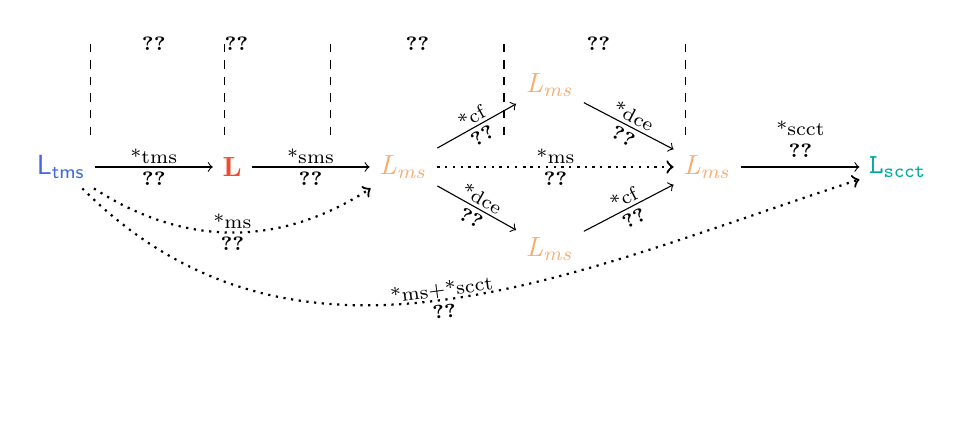
\begin{tikzpicture}
      \node (S) {$\src{L_{\tmssafe}}$};
      \node[right=1.5 of S] (T) {$\trg{L}$};
      \node[right=1.5 of T] (M) {$\irl{L_{\mssafe}}$};
      \node[below right=0.5 and 1.0 of M] (D0) {$\irl{L_{\mssafe}}$};
      \node[above right=0.5 and 1.0 of M] (C0) {$\irl{L_{\mssafe}}$};
      \node[right=3.0 of M] (E) {$\irl{L_{\mssafe}}$};
      \node[right=1.5 of E] (O) {$\obj{L_{\scctsafe}}$};

      \draw[->] (S) to[sloped] node[align=center,font=\scriptsize] (tmsedge) {\gls*{tms}\\ \Cref{thm:cca:rtp:tms}} (T);
      \draw[->] (T) to[sloped] node[align=center,font=\scriptsize] {\gls*{sms}\\ \Cref{thm:ccb:rtp:sms}} (M);
      \draw[->] (M) to[sloped] node[align=center,font=\scriptsize] {\gls*{dce}\\ \Cref{thm:ccdce:rtp:ms}} (D0);
      \draw[->] (M) to[sloped] node[align=center,font=\scriptsize] {\gls*{cf}\\ \Cref{thm:cccf:rtp:ms}} (C0);
      \draw[->] (D0) to[sloped] node[align=center,font=\scriptsize] {\gls*{cf}\\ \Cref{thm:cccf:rtp:ms}} (E);
      \draw[->] (C0) to[sloped] node[align=center,font=\scriptsize] {\gls*{dce}\\ \Cref{thm:ccdce:rtp:ms}} (E);
      \draw[->] (E) to[sloped,above] node[align=center,font=\scriptsize] {\gls*{scct}\\ \Cref{thm:ccscct:rtp:scct}} (O);

      % Sections
      \node[above=1.0 of tmsedge] (sectms) {{\scriptsize\Cref{subsec:cs:tms}}};
      \node[right=0.5 of sectms] (secsms) {{\scriptsize\Cref{subsec:cs:ms}}};
      \node[right=1.75 of secsms] (secopts) {{\scriptsize\Cref{subsec:cs:opts}}};
      \node[right=1.75 of secopts] (secscct) {{\scriptsize\Cref{subsec:cs:scct}}};

      \draw[thick,dotted,->] (S) to[bend right=33,sloped] node[align=center,font=\scriptsize] {\gls*{ms}\\ \Cref{thm:ccab:rtp:ms}} (M);
      \draw[thick,dotted,->] (M) to[bend right=0,sloped] node[align=center,font=\scriptsize] {\gls*{ms}\\ \Cref{thm:cccfccdce:rtp:ms}} (E);
      \draw[thick,dotted,->] (S) to[out=-45,in=198,sloped] node[align=center,font=\scriptsize] {\gls*{ms}+\gls*{scct}\\ \Cref{thm:ccall:rtp:msscct}} (O);

      \draw[dashed] ($(sectms)-(0.8,0)$) -- ($(sectms)-(0.8,1.25)$);
      \draw[dashed] ($(sectms)-(-0.9,0)$) -- ($(sectms)-(-0.9,1.25)$);
      \draw[dashed] ($(secsms)-(-1.2,0)$) -- ($(secsms)-(-1.2,1.25)$);
      \draw[dashed] ($(secscct)-(1.2,0)$) -- ($(secscct)-(1.2,1.25)$);
      \draw[dashed] ($(secscct)-(-1.1,0)$) -- ($(secscct)-(-1.1,1.25)$);
    \end{tikzpicture}
  \end{center}
  \caption{Visualisation of the optimising compilation pipeline that attains a combination of \gls*{ms} and \gls*{cct}. %
    Vertices in the graph are the programming languages from earlier sections (\Cref{sec:casestud:defs}). %
    All edges are secure compilers, but dotted edges use the presented framework (\Cref{sec:compcomp}) and strikethrough edges classic proof techniques. %
    The dashed lines partition the graph into the sections where the respective theorems are presented.
  }\label{fig:pipeline}
\end{figure}
The section demonstrates the power of the framework (\Cref{sec:compprop,sec:compcomp}) by composing these compilers for a secure and optimising compilation chain that robustly preserves \gls*{msscct}.
The first step in this chain is the compiler from $\src{L_{\tmssafe}}$ to $\trg{L}$ that robustly preserves just \gls*{tms} (\Cref{thm:cca:rtp:tms}).
From here, an instrumentation from $\trg{L}$ to $\irl{L_{\mssafe}}$ ensures that no out-of-bounds accesses can happen and, thus, programs at this point attain \gls*{sms} (\Cref{thm:ccb:rtp:sms}).
Since these properties compose into \gls*{ms}, composing these passes yields a compiler that robustly preserves \gls*{ms} (\Cref{thm:ccab:rtp:ms}).
At this stage, the section presents two optimising translations, namely \gls*{cf} and \gls*{dce}, each of which robustly preserves \gls*{ms} (\Cref{thm:ccdce:rtp:ms,thm:cccf:rtp:ms}).
These translations can be freely ordered in the compilation chain without compromising memory safety (\Cref{thm:cccfccdce:rtp:ms}).
The last step of the chain ensures that code stays \gls*{scct} (\Cref{thm:ccscct:rtp:scct}) when lowered from $\Lms$ to $\Lscct$.
The final result is that the whole compilation chain robustly preserves \gls*{msscct} (\Cref{thm:ccall:rtp:msscct}).



\subsection{Robust Temporal Memory Safety Preservation}\label{subsec:cs:tms}

This subsection defines a secure compiler from $\Ltms$ to $\Ltrg$.
To this end, the compiler needs to ensure that when execution switches from context to component, the type signatures are respected.
It can do so by inserting dynamic typechecks prior to entering the body of a function belonging to the component.

\begin{gather*}
  \begin{aligned}
    \cca(\src{x}) & = \trg{x} \\
    \cca(\src{n}) & = \trg{n} \\
    \cca(\src{\lbinop{\expr[_{1}]}{\expr[_{2}]}}) & =  \lbinop[\trg]{\left[\cca(\src{\expr[_{1}]})\right]}{\left[\cca(\src{\expr[_{2}]})\right]} \\
    \cca(\src{\lget{x}{\expr}}) & = \lget[\trg]{\trg{x}}{\left[\cca(\src{\expr})\right]} \\
    \cca(\src{\ldelete{x}}) & = \ldelete[\trg]{\left[\cca(\src{x})\right]} \\
%    \cca(\src{\lset{x}{\expr[_{1}]}{\expr[_{2}]}}) & = \lset[\trg]{\left[\cca(\src{x})\right]}{\left[\cca(\src{\expr[_{1}]})\right]}{\left[\cca(\src{\expr_{2}})\right]} \\
    \cca(\src{\lfunction{g}{x:\natt\to\type[_{e}]}{\expr}}) & = \lfunction[\trg]{\trg{g}}{\trg{x}}{\lifz[\trg]{\trg{\lhast{x}{\natt}}}{%
                                                                                                \left[\cca(\src{\expr})\right] %
                                                                                                 }{\labort[\trg]}}
  \end{aligned}
\end{gather*}

Since $\trg{L}$ has no static typechecks, it could happen that a bogus context $\trg{\library_{\ctx}}$ invokes a callable object accepting a $\src{\natt}$ with $\trg{\lpair{17}{29}}$.
By inserting the check, the compiler ensures that execution does not proceed in such cases.
The compiler does not insert other checks and proceeds as the identity function (which in this paper amounts to a simple re-colouring of $\src{L_{\tmssafe}}$ to $\trg{L}$ expressions).

Compiling the \texttt{strncpy} function from \Cref{sec:introduction} with $\cca$, the compiler would in this case ensure that the arguments that are evaluated in the compiled \texttt{strncpy} are valid.

\begin{theorem}[Compiler $\cca$ is secure with respect to \gls*{tms}]\label{thm:cca:rtp:tms}
  $\rtp{\cca}{\tmssafe}$ % \Coqed
\end{theorem}

\subsubsection{Proving Robust Safety Property Preservation}

\begin{figure}[!ht]
  \begin{center}
    \begin{tikzpicture}[state/.style={minimum height=1.5cm}]
      % relative horizontal/vertical distance between states
      \pgfmathsetmacro{\hdist}{0.95}
      \pgfmathsetmacro{\vdist}{1.35}
      \pgfmathsetmacro{\halfvdist}{0.725}

      % row of src states
      \node[state] (srcempty) {$\rtt{\src{\emptyset}}{\src{\lcall{main}{0}}}$};
      \foreach \s [remember=\s as \cur (initially empty)] in {1,w_1,p,w_2,2} {
        \node[state,right=\hdist of src\cur] (src\s) {$\rtt{\src{\Omega_{\s}}}{\src{\expr[_{\s}]}}$};
      }
      % row of trg states
      \node[state,below=\vdist of srcempty] (trgempty) {$\rtt{\trg{\emptyset}}{\trg{\lcall{main}{0}}}$};
      \foreach \s in {1,w_1,p,w_2,2} {
        \node[state,below=\vdist of src\s] (trg\s) {$\rtt{\trg{\Omega_{\s}}}{\trg{\expr[_{\s}]}}$};
      }
      %% illustrations
        % backtrans wrapper 1
        \draw[ultra thick,loosely dotted,Peach!50,rounded corners] (src1.north east) -- (srcw\string_1.north east)
          -- (trgw\string_1.south east) -- (trg1.south west) -- (src1.north west) -- cycle;
        % backtrans wrapper 2
        \draw[ultra thick,loosely dotted,Peach!50,rounded corners] (srcp.north east) -- (srcw\string_2.north east)
          -- (trgw\string_2.south east) -- (trgp.south west) -- (srcp.north west) -- cycle;
        % compiler correctness
        \draw[ultra thick,loosely dashed,Emerald!50,rounded corners] ($(srcw\string_1.north east)+(0,0.05)$) -- ($(srcp.north east)+(0,0.05)$)
          -- ($(trgw\string_2.north east)+(0.05,0)$) -- ($(trgw\string_2.south east)+(0.05,-0.05)$)
          -- ($(trg1.south west)+(-0.05,-0.05)$) -- ($(trg1.north west)+(-0.05,0)$) -- ($(srcw\string_1.north west)+(0,0.05)$) -- cycle;
      % state relations
      \path (srcempty) edge[very thick,draw=gray!25] node[pos=0.5,sloped,rotate=180,fill=white] {\scriptsize$\multimap_\emptyset$} (trgempty)
        (src1) edge[very thick,draw=gray!25] node[pos=0.5,sloped,rotate=180,fill=white] {\scriptsize$\multimap_{\delta_1}$} (trg1)
        (srcp) edge[very thick,draw=gray!25] node[pos=0.5,sloped,fill=white] {\scriptsize$\approx_{\delta_p}$} (trgp)
        (src2) edge[very thick,draw=gray!25] node[pos=0.5,sloped,rotate=180,fill=white] {\scriptsize$\multimap_{\delta_2}$} (trg2)
        (srcw\string_1) edge[very thick,draw=gray!25] node[pos=0.5,sloped,fill=white] {\scriptsize$\approx_{\delta_{w_1}}$} (trgw\string_1)
        (srcw\string_2) edge[very thick,draw=gray!25] node[pos=0.5,sloped,rotate=180,fill=white] {\scriptsize$\multimap_{\delta_{w_2}}$} (trgw\string_2)
        % diagonals
        (srcw\string_1) edge[thick,draw=gray!25] node[pos=0.16,sloped,rotate=180,fill=white] {\scriptsize$\approx_{\delta_{w_1}}$} (trg1)
        (src1) edge[thick,draw=gray!25] node[pos=0.16,sloped,rotate=180,fill=white] {\scriptsize$\multimap_{\delta_1}$} (trgw\string_1)
        (srcp) edge[thick,draw=gray!25] node[pos=0.2,sloped,fill=white] {\scriptsize$\approx_{\delta_p}$} (trgw\string_2)
        (trgp) edge[thick,draw=gray!25] node[pos=0.2,sloped,fill=white] {\scriptsize$\multimap_{\delta_{w_2}}$} (srcw\string_2)
        ;
      %\drawpolygon src1,srcw\string_1,trgw\string_1,trg1;
      %\drawpolygon srcp,srcw\string_2,trgw\string_2,trgp;
      %\node[font=\tiny,align=center,above=0.2 of srcw1srcp] (wrapper) {Backtranslation\\Wrapper};
      %\path[->,draw] (wrapper) -- (srcw\string_1);
      %\path[->,draw] (wrapper) -- (srcp);
      % steps
      \path[very thick,color=\stlccol] (srcempty) edge[draw=none] node {\ $\xrightarrow{\trace[_1]}{}{\kern-3.5pt}_{\text{ctx}}^*$} (src1)
        (src1) edge[draw=none] node {\ $\xrightarrow{\trace[_c]}{}{\kern-3.5pt}_{\text{ctx}}$} (srcw\string_1)
        (srcw\string_1) edge[draw=none] node {\ $\xrightarrow{\trace[_p]}{}{\kern-3.5pt}_{\text{ctx}}^*$} (srcp)
        (srcp) edge[draw=none] node[fill=white,inner sep=0,outer sep=0] {\ $\xrightarrow{\trace[_r]}{}{\kern-3.5pt}_{\text{ctx}}$} (srcw\string_2)
        (srcw\string_2) edge[draw=none] node {\ $\xrightarrow{\trace[_2]}{}{\kern-3.5pt}_{\text{ctx}}^*$} (src2)
        ;
      \path[very thick,color=\ulccol] (trgempty) edge[draw=none] node[fill=white,inner sep=0,outer sep=0] {\ $\xrightarrow{\phantom{\trace[_1]}}{}{\kern-3.5pt}_{\text{ctx}}^*$} (trg1)
        (trg1) edge[draw=none] node {\ $\xrightarrow{\phantom{\trace[_p]}}{}{\kern-3.5pt}_{\text{ctx}}^*$} (trgw\string_1)
        (trgw\string_1) edge[draw=none] node[fill=white,inner sep=0,outer sep=0] {\ $\xrightarrow{\phantom{\trace[_p]}}{}{\kern-3.5pt}_{\text{ctx}}^*$} (trgp)
        (trgp) edge[very thick,draw=none] node {\ $\xrightarrow{\phantom{\trace[_p]}}{}{\kern-3.5pt}_{\text{ctx}}^*$} (trgw\string_2)
        (trgw\string_2) edge[draw=none] node {\ $\xrightarrow{\phantom{\trace[_2]}}{}{\kern-3.5pt}_{\text{ctx}}^*$} (trg2)
        ;
      % legend
%     \node[align=left,below right=0.3 and 0.3 of trgempty,font=\tiny] (legend) {%
%       ${\src{\trace[_c]}}\cong{\backt{\Ltms}{\Ltrg}(\trg{Call\ ?\ foo\ \valueexpr})}$\\%
%       ${\src{\trace[_r]}}\cong{\backt{\Ltms}{\Ltrg}(\trg{Ret\ !\ foo\ \valueexpr})}$
%       };
      \node[below=0.5 of trgempty,draw=none] (legend) {};
      \draw[ultra thick,loosely dotted,Peach!50,rounded corners] ($(legend.north east)+(0.5,-0.4)$) -- ($(legend.north east)+(1,-0.4)$);
      \node at ($(legend.north east)+(1.5,-0.4)$) (legendwrapper) {};
      \node[right of=legendwrapper] {\tiny Backtranslation Wrapper};
      \draw[ultra thick,loosely dashed,Emerald!50,rounded corners] ($(legend.south east)+(0.5,0.4)$) -- ($(legend.south east)+(1,0.4)$);
      \node at ($(legend.south east)+(1.5,0.4)$) (legendcorrectness) {};
      \node[right of=legendcorrectness] {\tiny Compiler Correctness};
    \end{tikzpicture}
    \caption{Proof diagram for \Cref{thm:cca:rtp:tms} depicting the general structure of robust preservation proofs. %
      Nodes in the graph represent runtime states. %
      Vertical lines indicate cross language relations, while horizontal ones are execution steps. %
      The green dashed trapezoid encompasses the component segment, while the orange dotted rectangles entail the context switches. %
      $\Ltrg$ traces are omitted for readability. %
      $\Ltms$ trace segments $\src{\trace[_{c}]}$ and $\src{\trace[_{r}]}$ describe the events that happen at the boundaries, i.e., during a context switch.
      $\src{\trace_{p}}$ is the behavior of the component and the traces $\src{\trace[_{1}]}$ and $\src{\trace[_{2}]}$ describe the context.
    }\label{fig:proofdiag:rtp}
  \end{center}
\end{figure}


The proof of \Cref{thm:cca:rtp:tms} serves as boilerplate for proofs of the other secure compilation theorems of this paper.
Unfolding the statement gives the assumptions that for any $\pi\in\lceil\tmssafe\rceil$\footnote{$\lceil\cdot\rceil$ lifts the property to a hyperproperty by applying the powerset operation~\cite{clarkson2008hyper}.}, $\src{\trace}$, $\src{\runtimetermvar}$, and component $\src{\library_{comp}}$, $\rsat{\src{\library_{comp}}}{\pi}$ and $\progstepto{\prog[\trg]{\trg{\library_{\ctx}}}{\cca(\src{\library_{\comp}})}}{\trg{\runtimetermvar}}{\trg{\trace}}$, where $\trg{\library_{\ctx}}$ is arbitrary.
The proof obligation is $\msfilterL{\trg{\trace}}\in\pi$, i.e., the specification trace associated to $\trg{\trace}$ should satisfy the property $\pi$.
To show this, the trace $\trg{\trace}$ should be related with some $\Ltms$ trace $\src{\trace}$ and since there is a target execution associated to this trace, the task is to find an associated $\Ltms$ execution.
The trace $\trg{\trace}$ is split into different parts, where each part contains the events that either the context or the component does, but not both.
Because of this, all such trace segments are ,,well-bracketed'' in the sense that they start with either $\trg{\ev{Start}}$, $\trg{\ev{Call}\ \comptoctx\ foo\ \valueexpr}$, or $\trg{\ev{Ret}\ \comptoctx\ \valueexpr}$ and end with either $\trg{\ev{End}\ \valueexpr}$, $\trg{\ev{Ret}\ \ctxtocomp\ \valueexpr}$, or $\trg{\ev{Call}\ \ctxtocomp\ foo\ \valueexpr}$.
In the following, the former is referred to as a context segment, since, for these, execution happens in $\trg{\library_{\ctx}}$, and the latter as a component segment, since, for these, execution happens in $\cca(\src{\library_{\comp}})$.
\Cref{fig:proofdiag:rtp} visualises this split for a program execution with one call from context to component and how the target execution is related to a source execution.
In the figure, the green dashed lines encompass the component segments while the orange boxes contain the actual context switches from context to component or vice versa.
For the proof, it is necessary to know when two states $\src{\Omega}$ and $\trg{\Omega}$ are related.
Two cross-language relations make this precise: (i) $\multimap_{\delta}$ relates states that are involved in a context segment, allowing the target execution to perform internal calls, and (ii) $\approx_{\delta}$ relates states that are involved in a component segment, where both states need to agree exactly, i.e., the memory and the control flow states are required to contain the same information.
The relations are indexed with $\delta$, which is simply an injective mapping from $\Ltms$ locations $\src{\loc}$ to $\Ltrg$ locations $\trg{\loc}$.
Note that the relations $\multimap_{\delta}$ and $\approx_{\delta}$ swap when context switching.

So far, the paper explained how to relate an $\Ltms$ execution with the $\Ltrg$ execution at hand.
However, it is not yet demonstrated how the corresponding $\Ltms$ execution is actually built.
To do so, a trace-based backtranslation technique~\cite{abate2019jour} can be used to build a context $\src{\library_{\ctx}}$ that behaves similar to $\trg{\library_{\ctx}}$.
Since $\Ltms$ is statically typed, the context $\src{\library_{\ctx}}$ obtained from the backtranslation needs to be well-typed when linked with $\src{\library_{\comp}}$.
For context segments of the trace $\trg{\trace}$ it is also necessary to show that the execution behaves similarily, i.e., there is an $\Ltms$ trace segment $\src{\trace[']}$ that is related to the context segment, and that the states are related by $\multimap_{\delta}$.
When passing control to the component, the relatedness of states and traces follows from compiler correctness.
From all this, a source execution $\progstepto{\src{\prog{\library_{\ctx}}{\library_{\comp}}}}{\src{\runtimetermvar}}{\src{\trace}}$ can be obtained.

The proof now works as follows.
Rewrite the goal from $\msfilterL{\trg{\trace}}\in\pi$ to $\msfilterLtms{\src{\trace}}\in\pi$ after demonstrating that $\msfilterL{\trg{\trace}}=\msfilterLtms{\src{\trace}}$.
Then, specialize the robust satisfaction assumption $\rsat{\src{\library_{\comp}}}{\pi}$ to use the context $\src{\library_{\ctx}}$, which was obtained from backtranslating the context segments of the target trace $\trg{\trace}$, and the source execution $\progstepto{\src{\prog{\library_{\ctx}}{\library_{\comp}}}}{\src{\runtimetermvar}}{\src{\trace}}$.
This gives $\msfilterLtms{\src{\trace}}\in\pi$, which was to be demonstrated.

\subsection{Robust (Spatial) Memory Safety Preservation}\label{subsec:cs:ms}

\begin{center}
  $$
  \begin{array}{rcl}
    \ccb(\trg{\lnew{x}{\expr[_{1}]}{\expr[_{2}]}}) & = & \llet[\irl]{\irl{x_{SIZE}}}{\ccb(\trg{\expr[_{1}]})}{\lnew[\irl]{\irl{x}}{\irl{x_{SIZE}}}{\ccb(\trg{\expr[_{2}]})}} \\
    \ccb(\trg{\lget{x}{\expr}}) & = & \llet[\irl]{\irl{x_{n}}}{\ccb(\trg{\expr})}{\irl{\lifz{0\le x_{n}<x_{SIZE}}{\lget{x}{x_{n}}}{\labort}}} \\
    \ccb(\trg{\lset{x}{\expr[_{1}]}{\expr[_{2}]}}) & = & \llet[\irl]{\irl{x_{n}}}{\ccb(\trg{\expr[_{1}]})}{\lifz[\irl]{\irl{0\le x_{n}<x_{SIZE}}}{\lset[\irl]{\irl{x}}{\irl{x_{n}}}{\ccb(\trg{\expr[_{2}]})}}{\irl{\labort}}} \\
  \end{array}
  $$
\end{center}

The compiler $\cc{\trg{L}}{\Lms}$ only inserts bounds-checks whenever reading from or writing to memory in order to enforce \gls*{sms}.
For passing pointers, it has to pass them with their size information as well.
To this end, the compiler introduces another, fresh identifier $\irl{x_{SIZE}}$ for each allocation that binds $\irl{x}$ to keep track of the allocation size.
\begin{example}[Instrumented \texttt{strncpy}]
  Consider again \texttt{strncpy}, but instrumented for \gls*{sms}:
    \begin{lstlisting}[language=c,basicstyle=\ttfamily\small, morekeywords={size_t}]
  void strncpy(size_t n, size_t dst_size, char *dst,
                         size_t src_size, char *src) {
    for(size_t i = 0; i < src_size && src[i] != '\0' && i < n; ++i) {
      if(i < src_size && i < dst_size) {
        dst[i] = src[i];
      }
    }
  }
    \end{lstlisting}
    When calling this in similar fashion to \Cref{ex:strncpy:sms}, the event $\ev{Use}\ \loc_{x}\ 2;\comp;\unlock$ would not be emitted during execution, since the bounds check prevents the condition \texttt{src[i] != '\textbackslash 0'} from executing.
\end{example}

\begin{theorem}[Compiler $\ccb$ is secure with respect to \gls*{sms}]\label{thm:ccb:rtp:sms}
  $\rtp{\ccb}{\smssafe}$ % \Coqed
\end{theorem}

\Cref{thm:ccab:rtp:ms} states that the composition of $\cca$ and $\ccb$ is secure with respect to \gls*{ms} and follows from \Cref{thm:cca:rtp:tms,thm:ccb:rtp:sms} using \Cref{thm:rtp}.

\begin{theorem}[Compiler $\cca\circ\ccb$ is secure with respect to \gls*{ms}]\label{thm:ccab:rtp:ms}
  $\rtp{\cca\circ\ccb}{\mssafe}$ % \Coqed
\end{theorem}

\subsection{Optimising Compilers}\label{subsec:cs:opts}

\begin{gather*}
  \begin{align*}
    \ccdce(\irl{\lifz{true}{\expr[_{1}]}{\expr[_{2}]}}) & = \ccdce(\irl{\expr[_{1}]}) &\\
    \ccdce(\irl{\lifz{false}{\expr[_{1}]}{\expr[_{2}]}}) & = \ccdce(\irl{\expr[_{2}]}) &
  \end{align*}\\
  \begin{align*}
    \ccdce(\irl{\lbinop{\expr[_{1}]}{\expr[_{2}]}}) & = \lbinop[\irl]{\ccdce(\irl{\expr[_{1}]})}{\ccdce(\irl{\expr[_{2}]})} &
  \end{align*}\\[0.25cm]
  \begin{align*}
    \cccf(\irl{\expr}) & = \partialeval{\irl{\expr}}{\irl{\hole{\cdot}}} &
  \end{align*}\\[0.125cm]
  \begin{align*}
    \partialeval{\irl{x}}{\irl{\substlist}} & = \irl{n} & \text{if } \irl{\subst{n}{x}}\in\irl{\substlist} \\
    \partialeval{\irl{x}}{\irl{\substlist}} & = \irl{x} & \text{if } \irl{\subst{n}{x}}\notin\irl{\substlist} \\
    \partialeval{\irl{\lbinop{n}{m}}}{\irl{\substlist}} & = \irl{k} & \text{if } \lbinop{\irl{n}}{\irl{m}}=k \\
%    \partialeval{\irl{\lbinop{\expr[_{1}]}{\expr[_{2}]}}}{\irl{\substlist}} & = \lbinop[\irl]{\partialeval{\irl{\expr[_{1}]}}{\irl{\substlist}}}{\partialeval{\irl{\expr[_{2}]}}{\irl{\substlist}}} \\
    \partialeval{\irl{\llet{x}{n}{\expr}}}{\irl{\substlist}} & = \partialeval{\irl{\expr}}{\irl{\subst{x}{n}},\irl{\substlist}} \\
    \partialeval{\irl{\lget{x}{\expr}}}{\irl{\substlist}} & = \lget[\irl]{\irl{x}}{\partialeval{\irl{\expr}}{\irl{\substlist}}}
  \end{align*}\\
  \begin{align*}
    \partialeval{\irl{\llet{x}{\expr[_{1}]}{\expr[_{2}]}}}{\irl{\substlist}} & = \llet[\irl]{\irl{x}}{\partialeval{\irl{\expr[_{1}]}}{\irl{\substlist}}}{\partialeval{\irl{\expr[_{2}]}}{\irl{\substlist}}} \\
    \partialeval{\irl{\lifz{\expr[_{1}]}{\expr[_{2}]}{\expr[_{3}]}}}{\irl{\substlist}} & = \lifz[\irl]{\partialeval{\irl{\expr[_{1}]}}{\irl{\substlist}}}{\partialeval{\irl{\expr[_{2}]}}{\irl{\substlist}}}{\partialeval{\irl{\expr[_{3}]}}{\irl{\substlist}}} \\
  \end{align*}
\end{gather*}

The two optimising compiler passes from $\Lms$ to $\Lms$ perform \gls*{dce} and \gls*{cf}, respectively.
The \gls*{dce} pass applies a naive rewrite rule on conditionals.
For \gls*{cf}, the pass uses an auxiliary function \texttt{mix} that does the actual work.
It rewrites constant binary operations, e.g., $\irl{{17}+{29}-1}$ to $\irl{46-1}$, and replaces variables that are assigned to constants with their constant, e.g., $\irl{\llet{x}{7}{x}}$ to $\irl{7}$.
Both passes are secure with respect to \gls*{ms}.
The proof for either is relatively simple, because both \gls*{dce} and \gls*{cf} do not change the way memory accesses happen.
Moreover, since the input and output languages to these compilers are the same, attacker contexts do not have more power in the target language than in the source.

\begin{theorem}[Compiler $\ccdce$ is secure with respect to \gls*{ms}]\label{thm:ccdce:rtp:ms}
  $\rtp{\ccdce}{\mssafe}$ %\Coqed
\end{theorem}
\begin{theorem}[Compiler $\cccf$ is secure with respect to \gls*{ms}]\label{thm:cccf:rtp:ms}
  $\rtp{\cccf}{\mssafe}$ %\Coqe
\end{theorem}

With both \Cref{thm:ccdce:rtp:ms,thm:cccf:rtp:ms} it follows from \Cref{corr:swappable} that the two passes can be interchanged arbitrarily:

\begin{theorem}[Compilers $\cccf\circ\ccdce$ and $\cccf\circ\ccdce$ are secure with respect to \gls*{ms}]\label{thm:cccfccdce:rtp:ms}
  $\rtp{\cccf\circ\ccdce}{\mssafe}$ and $\rtp{\ccdce\circ\cccf}{\mssafe}$. % \Coqed
\end{theorem}

\subsection{Robust Strict Cryptographic Constant Time Preservation}\label{subsec:cs:scct}

\begin{center}
  \begin{align*}
    \ccscct(\irl{\lfunction{g}{x}{\expr}}) & = \lfunction[\obj]{\obj{g}}{\obj{x}}{\obj{\lwrdoit{1};}\ccscct(\irl{\expr})} \\
    \ccscct(\irl{\lcall{g}{\expr}}) & = \lcall[\obj]{\obj{g}}{\ccscct(\irl{\expr})\obj{; wrdoit{1}}} \\
    \ccscct(\irl{\lbinop{\expr[_{1}]}{\expr[_{2}]}}) & = \lbinop[\obj]{\ccscct{\irl{\expr[_{1}]}}}{\ccscct{\irl{\expr[_{2}]}}} \\
  \end{align*}
\end{center}

Given the fact that $\Lscct$ provides a \gls*{cct}-mode that can be turned on or off, the compiler inserts wrapper code for function bodies to ensure that execution in the component always happen in this \gls*{cct}-mode.
The context can overwrite the flag and exit the mode, but upon invoking a function that is part of the component, the flag would be set again.
Because of this, the compiler is secure with respect to \gls*{scct}, similarly proven as in \Cref{subsec:cs:tms}.

\begin{theorem}[Compiler $\ccscct$ is secure with respect to \gls*{scct}]\label{thm:ccscct:rtp:scct}
  $\rtp{\ccscct}{\scctsafe}$ % \Coqed
\end{theorem}

\subsection{Robust Preservation of Intersection of Memory Safety and Strict Cryptographic Constant Time}

Let $\ccmsscct$ be the compiler that is the composition of $\cca$, $\ccb$, $\cccf$, $\ccdce$, and $\ccscct$, then the following theorem holds.

\begin{theorem}[Compiler $\ccmsscct$ is secure with respect to \gls*{scct}]\label{thm:ccall:rtp:msscct}
  $\rtp{\cc{\Ltms}{\Lscct}}{\mssafe\cap\scctsafe}$ \Coqed
\end{theorem}
\begin{proof}
	From \Thmref{thm:ccscct:rtp:scct}, we have that any LTMS program $\src{p}$ gets compiled into a L program $\trg{p}$ that is also TMS.
	Then, from \Thmref{thm:cccfccdce:rtp:ms} we have that $\trg{p}$ gets compilet to a program ?? that is also SMS, assuming it was SMS to begin with.
	Since TMS + SMS = MS, ?? is MS.
	?? gets optimised by the optimisation passes and its optimisation is ???, which is still MS.
	Finally, \Thmref{thm:ccab:rtp:ms} ensures that ??? gets compiled into ????, which is CCT assuming that the original program was CCT to begin with.
	\MPin{please fill in the macros here}
  % \MKin{%
  %   \textbackslash Thmref or \textbackslash Cref?
  % }
% Unfold the definition of $\rtp{\cc{\Ltms}{\Lscct}}{\mssafe\cap\scctsafe}$.
% So, let $\pi\in\mssafe\cap\scctsafe$, $\src{\progvar}$ such that $\rsat{\src{\progvar}}{\pi}$ and let $\obj{\contextvar},\obj{\runtimetermvar}$ with $\progstepto{\prog[\obj]{\obj{\contextvar}}{\left(\cc{\Ltms}{\Lscct}(\src{\progvar})\right)}}{\obj{\runtimetermvar}}{\obj{\trace}}$.
% What is left to show is $\scctfilterLscct[\emptyset]{\obj{\trace}}\in\pi$.
% Let $\irl{\progvar}=\cc{\Ltms}{\Ltrg}\circ\cc{\Ltrg}{\Lms}\circ\cc[\gls*{cf}]{\Lms}{\Lms}\circ\cc[\gls*{dce}]{\Lms}{\Lms}(\src{\progvar})$ such that $\cc{\Lms}{\Lscct}(\irl{\progvar})=\cc{\Ltms}{\Lscct}(\src{\progvar})$.
% Note that $\pi\in\scctsafe$, so apply \Thmref{thm:ccscct:rtp:scct}
\end{proof}

\section{Related Work\pages{2}}\label{sec:relwork}

This section discusses work on robust compilation (\Cref{subsec:relw:seccomprtp}) and on other secure compilation criteria (\Cref{subsec:relw:seccompcrit}).
Since the case study of \Cref{sec:casestud:defs,sec:casestud:rtp} implements measures for preserving \gls*{ms} and \gls*{cct}, this section then presents relevant related work as well (\Cref{subsec:relw:msmechs,subsec:relw:cctmechs}).

\subsection{Secure Compilation as Robust Preservation}\label{subsec:relw:seccomprtp}

The robust preservation of properties as a compiler-level criterion has been analyzed extensively~\cite{abate2019jour,patrignani2021rsc,abate2021extacc,patrignani2019survey} and thus we build on that framework.
No existing work is concerned with composing robustly safe compilers.
These works consider languages with different trace models and our technical setup can be adapted to that as long as security properties and their monitors are still defined on the same trace model.
The work relating robust preservation with universal composability~\cite{patrignani2022universal} is closest to what this paper presents.
The authors demonstrate a similar compositionalty theorem to what is presented here (\Cref{sec:compcomp}) but use it in the context of protocols.
They do not demonstrate the scalability of the approach.
Moreover, they are missing the upper and lower compositions.
% The authors demonstrate a similar compositionality theorem to what is presented here (\Cref{sec:compcomp}) as well as in an earlier version of this work~\cite{kruse2022csc}.
% However, they do not demonstrate the scalability of the approach by means of a case study.

\subsection{Other Secure Compilation Criteria}\label{subsec:relw:seccompcrit}

While this paper focuses on the robust preservation framework~\cite{abate2019jour}, other secure compilation criteria exist.
The survey on formal approaches to secure compilation~\cite{patrignani2019survey} discusses a broad spectrum already, while this section presents a very high-level overview.
Fully abstract compilation~\cite{abadi1999fullabstraction} states that a compiler should preserve and reflect observational equivalence between source and target programs.
It was shown~\cite{abate2021faandrc} that fully abstract compilers robustly preserve program properties that are either trivial or meaningless.
As a mitigation for this, the authors presented a categorical approach based on maps of distributive laws~\cite{watanabe2002modl}, which they call many maps of distributive laws.
Maps of distributive laws have been investigated before as a possible secure compilation criterion~\cite{tsampas2020catsc}.
Other approaches are extensions of the compiler correctness criterion as discussed in other work~\cite{patterson2019next700} or the introduction of opaque observations~\cite{vu2021reconciling} to reconcile compiler optimisations with security.
Note that this work also presents secure compilers that are optimising, but contrary to the other~\cite{vu2021reconciling}, provides a formal account of these in the robust preservation framework.
% Lastly, the authors of this paper have presented ongoing work~\cite{patrignani2023blame} on a weaker robust preservation criteria based on the concept blame.

\subsection{Memory Safety Mechanisms}\label{subsec:relw:msmechs}

Different mechanisms for enforcing memory safety exist that also consider the secure compilation domain, i.e., have an active attacker model.
For example, the ,,pointers as capabilities'' principle represents pointers as machine-level capabilities~\cite{korashy2021capableptrs}, which behave in a similar fashion to capabilities by means of linear typing~\cite{morrisett2005L3}.
The approach of this paper also uses linear typing, but differs from $L^{3}$~\cite{morrisett2005L3} in the way that functions are not first-class.
Moreover, this paper considers an active attacker, while the work on $L^{3}$ only discusses whole programs and, thus, has no active attacker model.
The instrumentation to ensure memory safety that this paper presents is inspired by Softbounds~\cite{nagarakatte2009soft}.
That work inserts bounds-checks in front of pointer-dereferences and, for this to work, inserts meta-data information on pointer creation.
Softbounds also works in a more advanced setting with structured fields accesses and also introduces a table-lookup for pointers that are stored in memory.
This paper only considers arrays of primitive data, i.e., there are no pointers to pointers or structures.
Several other approaches to memory-safety exist in literature, specifically as compiler instrumentations~\cite{akritidis2009baggy,younan2010paricheck,jung2021pico,shankaranarayana2023tailcheck,dhumbumroong2020boundwarden,nam2019framer,zhou2023fatptrs}, hardware-extensions~\cite{kwon2013lowfat,saileshwar2022heapcheck,chen2023flexpointer,kim2023whistle}, or programming language extensions~\cite{elliott2018checkedc,li2022formalcheckedc,jim2002cyclone,elliott2015guilt,west2005cuckoo,weis2019fyr,benoit2019uniqueness}.
What differentiates this work from them is that this work uses known, compiler-based approaches to ensure memory-safety as a means to investigate secure compiler compositions.
This paper does not provide efficient memory-safety, but serves as a theoretical foundation for the secure compilation domain.

To extend the languages in this paper with a less restricted form of pointer arithmetic, the region coloring memory safety monitor presented in earlier work~\cite{michael2023mswasm} can be used.
The work presenting this monitor provides an approach for the robust preservation of memory safety compiling from C to WASM.
However, they do not discuss composition of secure compilers but rather investigate an instance of a secure compiler.

\subsection{Cryptographic Constant Time Mechanisms}\label{subsec:relw:cctmechs}

The approach to preserving cryptographic constant time in this paper is high-level, where a programming language exposes a way to switch the semantics to a data (operand) independent timing mode.
Since identifiers in $\Lscct$ are annotated with a secrecy tag, this approach is similar to others with information flow control.
For example, Vale~\cite{bond2017vale} uses Dafny to ensure constant-time assembly code, while Jasmin~\cite{almeida2017jasmin} makes use of the Coq proof assistant to reject non-constant-time programs.
CT-Wasm~\cite{watt2019ctwasm} enforces constant-timeness by means of a type system.
Different to the approach of this paper, these approaches necessitate that the programmer writes \gls*{cct} code.
An approach to allow programmers to write more high-level code is CryptOpt~\cite{kuepper2023cryptopt}, which generates efficient target-code by means of a randomised search.
This paper abstracts over concrete mitigation strategies and simply assumes that there is a flag to switch to a cryptographic-constant time execution mode.
This can be realised by employing the FaCT~\cite{cauligi2019fact} compiler, which translates common non-constant time code patterns to be constant-time, and the data (object) independent timing execution mode of modern processors.

\section{Conclusion\pages{$\sfrac{1}{2}$}}\label{sec:concl}
This paper tackled the problem of understanding what kind of security properties does a secure compiler preserve, when said compiler is the combination of smaller compiler passes that preserve possibly different security properties.
% 
For this, this paper first formalised security properties of interest and their composition.
% 
Then, it proved that composing secure compilers that preserve certain properties results in a secure compiler that preserves the composition of the properties.
% 
Finally, this paper defines a multi-pass compiler and proves that it preserves \gls*{msscct}.
Crucially, this paper derives the security of the multi-pass compiler from the composition of the security properties preserved by its individual passes, which include security-preserving as well as optimisation passes.


% This paper does a first step towards practical secure compilation chains by introducing a theoretical framework demonstrating that secure compilers compose.
% The paper exercises this framework on a case-study that consists of an optimising compilation chain that is secure with respect to \gls*{msscct}.
% \MP{
% 	not an appropriate recap.
% 	rewrite summarising the paper
% }

% In future work, it would be interesting to investigate whether it is possible to provide {\em secure compiler combinators}, similarly to how parser combinators work.
% %To this end, it may be necessary to extend existing frameworks for multi-language semantics.
% It is also interesting to extend our case-study and verify all results of it in Coq.
% This way, it is possible to obtain an executable, secure compiler.
% However, the formalisation effort for backtranslation proofs is known to be enormous\MP{cit + details}, so another research avenue may be to find better ways to (semi-)automate standard secure compilation proofs.
% \MPin{
% 	not particularly informative FW. i'd rather not have it as such
% }

%% The acknowledgments section is defined using the "acks" environment
%% (and NOT an unnumbered section). This ensures the proper
%% identification of the section in the article metadata, and the
%% consistent spelling of the heading.

% \begin{acks}
%   We would like to thank the anonymous reviewers for their feedback.
% 	This work was partially supported by a gift from
		% the Italian Ministry of Education through funding for the Rita Levi Montalcini grant (call of 2019).
% \end{acks}

\newpage
%%
%% The next two lines define the bibliography style to be used, and
%% the bibliography file.
\bibliographystyle{ACM-Reference-Format}
\bibliography{main}

%%
%% If your work has an appendix, this is the place to put it.
\appendix

\end{document}
\endinput
%%
%% End of file `sample-sigconf.tex'.
